\chapter{Variable Topology}
\minitoc
\section{Introduction}
In the previous chapter all numerical scheme were done on the same domain.
We will here see the change that we need to make if we want to have variable topology.


We will need to take care of two additional thing:
\begin{enumerate}
\item Know the speed in cell that weren't in the domain but are in the new time step.
\item Know the position of the different boundary.
\end{enumerate}

We are mainly interested in mobile boundary consisting in free surface boundary because it will be the only
boundary that move depending on the solution.

The motion of the domain and the boundary is given by:
\begin{equation}
\dot{\vect{x}}=\vect{v}
\end{equation}

Where $\vect{v}$ is the speed at the given position.

To discretize this equation, we will use particle  placed in every cell. A cell where a particle lie is in the domain.
A cell without particle is out of the domain.

But particle move with the speed given at there position, witch is not on a grid point.

Because of this, we need to interpolate the speed at the given point.

When a particle move to a new cell, we need to know the initial speed at this position.
We analytically have boundary condition for speed at boundary.
We need to extrapolate this boundary condition one cell away.

\section{Analytical equation}

We can write a none discretized particle method equation as:

\begin{align*}
	\dot{v}&=\left(\eye + P(D(\vect{x}))\right)f(\vect{v},\vect{x})\\
	\dot{x}&=v
\end{align*}

Where $x$ are a continuous representation of the space with particle.
The notation $P(D(\vect{x}))$ say that we consider the projection operator with boundary condition given by $D(\vect{x})$.

We need to add to this boundary condition, that are given by a linear differential operator $A$.
\begin{equation}
	A\vect{v}=0
\end{equation}
$A$ contain derivative with respect to space but not respect to time.

When we discretize, we will need to interpolate because we need speed at position we don't know (for a staggered grid we have):
\begin{align*}
	\left.\dot{\vect{v}}\right|_{\in D_{v}(D(\vect{x}))}&=\left(\eye+P(D(\vect{x}))\right)\left.f(E(\vect{v},D_v(D(\vect{x}))),D_{v}(D(\vect{x})))\right|_{\in D_{v}(D(\vect{x}))}\\
	\dot{x}&=I\left(\vect{x},E(\vect{v},D_v(D(\vect{x})))\right)\\
	\left.\vect{v}\right|_{\notin D_{v}(D(\vect{x}))}&=\left.E(\vect{v},D_v(D(\vect{x})))\right|_{\notin D_{v}(D(\vect{x}))}
\end{align*}

For mathematical simplicity we will take that $\vect{v}$ consist of a speed defined everywhere, 
but in the computation only speed that are accessed in the time step is needed (only speed in the domain and in it's neighbour).
We can model this by considering none used cell with a special value like nan that propaget contagious in every operation.

\begin{description}
\item[$D(\vect{x})$] indicate the domain in witch at least a particle is found. This consist at the same time to the topology for pressure (Pressure are cell centered).
\item[$D_{v}$] is a function depending of the topology given in general by $D(\vect{x})$ and indicate witch speed component are in the domain.
\item[$f$] is a function that take as argument the topology for pressure given by $D(\vect{x})$ and the topology for speed given by $D_v(D(\vect{x}))$ and the speed everywhere.
\item[$E$] is the extrapolation operator witch take as argument the speed everywhere and return a speed everywhere,
but where the speed in the speed domain is not changed. This speed is the speed that the fluid had if it where there.
The distance to witch this extrapolation operator need to give value depend on the choice of the time step.
The extrapolation operator need to take account of two thing:
\begin{enumerate}
	\item The correct boundary condition.
	\item Extrapolate speed farther away than the boundary condition if a particle move more than one cell, or if boundary condition doesn't give constraint of a given cell.
\end{enumerate}

\item[$I$] is an interpolation operator witch from the speed at discrete position find the speed at a given position.
\end{description}

The use of two topology is needed because in a staggered grid the position of speed and pressure is not the same.

\begin{remark}
$D_{v}$ need to be good chosen to avoid pathological case.
For example for a cell with only one cell. We will normally consider all speed as boundary. But with only boundary we have no speed data.
For this reason in this case, we consider all boundary cell as in the domain.
\end{remark}


\subsection{Splitting}
\label{splitting}

A simple but of only order $1$ (in general) mean to solve this equation, is to consider two different problem:
\begin{enumerate}
	\item Advance speed for a given topology.
	\item Advance the particle from the given speed.
\end{enumerate}

The first step is to solve:
\begin{align}
\left.\dot{\vect{v}}\right|_{\in D_{v}(D(\vect{x}))}&=\left(\eye+P(D(\vect{x}))\right)\left.f(E(\vect{v},D_v(D(\vect{x}))),D_{v}(D(\vect{x})))\right|_{\in D_{v}(D(\vect{x}))}\\
	\left.\vect{v_{t_0}}\right|_{\notin D_{v_{t_0}}(D(\vect{x}))}&=\left.E(\vect{v_{t_0}},D_v(D(\vect{x})))\right|_{\notin D_{v}(D(\vect{x}))}
\end{align}

Witch can be done like in the fixed topology case with a Runge-Kutta method. The second equation indicate the boundary condition.
Numerically we can calculate the speed at boundary at every evaluation of $f$.

We then move the particle with the calculated speed.
\begin{equation}
	\dot{x}=I\left(\vect{x},E(\vect{v},D_v(D(\vect{x})))\right)\\
\end{equation}

This method is only of order 1.
We can see it from the following example:
\begin{example}
Consider only one particle. With as initial condition 0 speed without viscosity.

The extrapolation operator in this case will copy the speed vertically,
the speed will be constant and the only none zero component is in the $y$ direction.
The speed will be given by the integration of the gravity force, the convective term is 0 because speed is constant.
The speed will be calculated with an accuracy of order of the Runge-Kutta method used (4 for rk4).
But the position will be calculated from the advance of a constant speed for every time step. This is then equivalent to the euler
method of order 1.

In final, our speed will be correct at order $k$ but position will be wrong.

This error doesn't depend on the precision of integration for the speed or position problem.
It come from the splitting.
\end{example}

\subsection{One differential equation}
\label{differentialequation}
We will now show how we can rewrite this differential equation in only differential equation.
For this, we need an expression for the derivative of the boundary condition.
When we have it, we only have to use a Runge-Kutta method.


We will now only be interested in the case where $E$ is a linear operator white the two following constraint:
\begin{itemize}
	\item It's effect for speed in the domain (for speed) is the identity.
	\item It's effect for speed out of the domain (for speed) depend only on speed of the domain (for speed).
\end{itemize}

The domain for speed for $E$ is noted $E(D_v(D(\vect{x})))$.

In matrix notation it tell that some block need to be $0$ or $\eye$.
If we consider that indice from $1$ to $n_d$ are in the domain(for speed) and $n_d+1$ to $n$ are out of the domain (for speed), the constraint for a line of the matrix is,
using as notation the : as in matlab in indicating by an indice it's position in the vector:
\begin{align}
	\intertext{For $i<n_d+1$}
	E_{i :}&=\left( 0 \ldots 1_{i} \ldots 0\right)\\
	\intertext{For $i>n_d$}
	E_{i :}&=\left( e^i_{1}\ldots e^i_{n_d} 0\ldots 0\right)\\
\end{align}

Taking the derivative of $E(D_v(D(\vect{x})))\vect{v}$ has two term, the first give:
\begin{equation}
	E(D_v(D(\vect{x})))\dot{\vect{v}}
\end{equation}

Witch use $\dot{\vect{v}}$ but need it only for the domain because outside the given column of the $E$ matrix is zero.

The second therm is the derivative of the matrix $E$ with respect of change of time. Witch will lead to the derivative with respect of change of topology.
This will give a delta of dirac.

The reason of this is because of the discontinuity in time of the boundary speed, when we change topology.

We will neglect this dirac delta. The equation is then:
\begin{align}
	\left.\dot{\vect{v}}\right|_{\in D_{v}(D(\vect{x}))}&=\left(\eye+P(D(\vect{x}))\right)\left.f(E(D_v(D(\vect{x})))\vect{v},D_{v}(D(\vect{x})))\right|_{\in D_{v}(D(\vect{x}))}\\
	\left.\dot{\vect{v}}\right|_{\notin D_{v}(D(\vect{x}))}&=E(D_v(D(\vect{x})))\left(\eye+P(D(\vect{x}))\right)\left.f(E(D_v(D(\vect{x})))\vect{v},D_{v}(D(\vect{x})))\right|_{\in D_{v}(D(\vect{x}))}\\
	\left.\vect{v_{t_0}}\right|_{\notin D_{v_{t_0}}(D(\vect{x}))}&=\left.\left(E(D_v(D(\vect{x})))\left.\vect{v_{t_0}}\right|_{\in D_{v}(D(\vect{x}))}\right)\right|_{\notin D_{v}(D(\vect{x}))}\\
	\dot{x}&=I\left(\vect{x},E(D_v(D(\vect{x})))\vect{v}\right)\\
\end{align}
Where we have used the notation that vector can be extended with 0 when needed because the extension is not needed because the good column are zero.

Witch can be rewritten as:
\begin{align}
	\dot{\vect{v}}&=E(D_v(D(\vect{x})))\left(\eye+P(D(\vect{x}))\right)\left.f(E(D_v(D(\vect{x})))\vect{v},D_{v}(D(\vect{x})))\right|_{\in D_{v}(D(\vect{x}))}\\
	\left.\vect{v_{t_0}}\right|_{\notin D_{v_{t_0}}(D(\vect{x}))}&=\left.\left(E(D_v(D(\vect{x})))\left.\vect{v_{t_0}}\right|_{\in D_{v}(D(\vect{x}))}\right)\right|_{\notin D_{v}(D(\vect{x}))}\\
	\dot{x}&=I\left(\vect{x},E(D_v(D(\vect{x})))\vect{v}\right)\\
\end{align}
Where we have used that $E$ is the identity in the domain.

This equation can be integrated with a Runge-Kutta method.
For having a maximal precision, the boundary speed is taken from the extrapolation at every complete Runge-Kutta step.

In the argument of $f$ we have used an extrapolation of speed witch don't depend of the input in boundary speed (because the $E$ matrix has zero column where needed).
The integrated boundary speed is only used in the case where a cell become in the domain in a time step.

The neglected dirac delta will only have an effect on a boundary speed component in the case where in a Runge-Kutta step the following happen:
\begin{enumerate}
	\item A neighbor cell(cell witch $E$ matrix has component with) fill.
	This will change the value of boundary speed with a jump (this jump will be neglected).
	\item The given speed is used because a particle fill the domain.
	This is needed because in the contrary the speed calculated will not be used.
\end{enumerate}

This effect will change the precision when it happen from order $k$ to order 1.
And this error will only be on the boundary condition being not exactly respected for a short time.
The force will be integrated correctly.

The direct filling of a cell don't pose problem because we don't have discontinuity in speed, because in the first region we force speed,
in the second the derivative.

The jump is only caused because we force speed differently for the two region witch give a discontinuity.

We consider the same example than before:
\begin{example}
One particle with 0 initial speed, without viscosity.
The speed will be constant. So only the gravity force act and the extrapolation operator will copy speed vertically.
The result will then be equivalent to the integration of the purely particle problem where the speed change is calculated at particle position.
The order of the method is then $k$.
\end{example}
\section{Extrapolation}

We will now discuss how to define the extrapolation operator.

We have seen that the extrapolation operator need to do two thing:
\begin{enumerate}
	\item Ensure correct boundary condition.
	\item Extrapolate the rest of speed.
\end{enumerate}

We now are interested in the ensuring of boundary condition.

Numerically this will be done in extrapolating the value at exterior from the boundary condition on the derivative.

One important point is how we enforce the boundary condition in discretized grid.

In the boundary we have (for 3d case):
\begin{align}
	\sum_{i,j}\sigma_{ij}n_{i}n_{j}&=0\\
	\sum_{i,j}\sigma_{ij}t^{1}_{i}n_{j}&=0\\
	\sum_{i,j}\sigma_{ij}t^{2}_{i}n_{j}&=0\\
\end{align}

$\vect{n}$ is the normal vector of the surface.
$\vect{t}^{1}$ and $\vect{t}^{2}$ are none colinear tangent vector.

In 2d we only have only one tangent vector.

$\sigma_{ij}$ is given by:
\begin{equation}
	\sigma_{ij}=-p \delta_{ij}+\nu\left(\frac{\partial v_{i}}{\partial x_{j}}+\frac{\partial v_{j}}{\partial x_{i}}\right)
\end{equation}

The first equation can be used to find boundary condition for $p$.
With:
\begin{equation}
	p=O(\nu)
\end{equation}

$\nu$ is small for water ($\approx 10^{-6}$. This justify the often used boundary condition of 0.

The other equation only depend of speed, because $\vect{n}$ is orthogonal to $\vect{t}^{1}$ and $\vect{t}^{2}$.
The value of $\nu$ is not relevant for the condition (a global none zero constant).
The constraint is linear. With sufficiently equation and know value we can find an unique solution.

We now will treat the different possible case in 2d. This will then be generalized in 3d.

We will use different discretisation point for pressure and speed.
We begin with the discretisation for speed.

\subsection{2d}
\label{topo:extrap:2d}
\subsubsection{Plane}

The first case is a surface witch is a plane following one of the cell boundary.

Without loss of generality we consider the plane in the $x$ direction(the other case are isometrie of this case).

The normal and tangent vector are then given by:
\begin{align}
	\vect{n}&=\begin{pmatrix}
			0\\
			1
		\end{pmatrix}\\
	\vect{t}&=\begin{pmatrix}
			1\\
			0
		\end{pmatrix}
\end{align}

The equation are then given by:
\begin{align}
	\sum_{i,j}\sigma_{ij}t_{i}n_{j}&=0\\
	\sigma_{12}&=0\\
	-p \delta_{12}+\nu\left(\frac{\partial v_{1}}{\partial x_{2}}+\frac{\partial v_{2}}{\partial x_{1}}\right)&=0\\
	\frac{\partial v_{1}}{\partial x_{2}}+\frac{\partial v_{2}}{\partial x_{1}}&=0\\
\end{align}

We discretize this equation at point $i+\frac{1}{2},j+\frac{1}{2}$:
\begin{equation}
\label{var:extr:droitCont}
	\frac{v^{1}_{i+\frac{1}{2},j+1}-v^{1}_{i+\frac{1}{2},j}}{\Delta x_{2}}+\frac{v^{2}_{i+1,j+\frac{1}{2}}-v^{2}_{i,j+\frac{1}{2}}}{\Delta x_{1}}=0
\end{equation}

Where $\Delta x_{1}$ and $\Delta x_{2}$ are the spacing in $x$ and $y$.
We have one equation for 3 unknows, only $v^{1}_{i+\frac{1}{2},j}$ are know.
But we can add two equation using the divergence free condition in the fluid for cell $i,j$ and $i+1,j$.

This give us:
\begin{align}
\label{var:extr:droitContA}
	0&=\frac{v^{1}_{i+\frac{1}{2},j}-v^{1}_{i-\frac{1}{2}},j}{\Delta x_{1}}+\frac{v^{2}_{i,j+\frac{1}{2}}-v^{2}_{i,j-\frac{1}{2}}}{\Delta x_2}\\
\label{var:extr:droitContB}
	v^{2}_{i,j+\frac{1}{2}}&=v^{2}_{i,j-\frac{1}{2}}-\frac{v^{1}_{i+\frac{1}{2},j}-v^{1}_{i-\frac{1}{2},j}}{\Delta x_{1}}\Delta x_{2}\\
\label{var:extr:droitContC}
	0&=\frac{v^{1}_{i+\frac{3}{2},j}-v^{1}_{i+\frac{1}{2}},j}{\Delta x_{1}}+\frac{v^{2}_{i+1,j+\frac{1}{2}}-v^{2}_{i,j-\frac{1}{2}}}{\Delta x_2}\\
\label{var:extr:droitContD}
	v^{2}_{i+1,j+\frac{1}{2}}&=v^{2}_{i+1,j-\frac{1}{2}}-\frac{v^{1}_{i+\frac{3}{2},j}-v^{1}_{i+\frac{1}{2},j}}{\Delta x_{1}}\Delta x_{2}
\end{align}

We substitute the two equation \ref{var:extr:droitContB} and \ref{var:extr:droitContD} in equation \ref{var:extr:droitCont}.
Witch will now only depend on one unknows $v^{1}_{i+\frac{1}{2},j+1}$ witch depend on quantity that can be found using the speed in the domain.

Figure \ref{topology:extrap:plane} show the variable used and witch are substitute from other.

We can only do the thing that we have done only if we have a depth of minimal two cell.
If we have only one cell, we have no $y$ speed in the domain in calculation.
For this case, consider the speed $y$ at boundary as in the domain at let it evolve without constraint.

\begin{figure}
\directlua{dofile('topology/plane_extrapolation.lua')}
\caption{The red point is the place where the boundary condition is discretized.
The green dot are cell where the divergence free rule is enforced. Red vector are calculated with respect of the blue one.}
\label{topology:extrap:plane}
\end{figure}

\subsubsection{\unit{45}{\degree} Plane}

If we have a cell in domain with two adjacent cell witch are not in the domain.
We take as normal a \unit{45}{\degree} Plane.

The normal and tangent vector are then:
\begin{align}
	\vect{n}&=\begin{pmatrix}
	\frac{\sqrt{2}}{2}\\
	\frac{\sqrt{2}}{2}
	\end{pmatrix}\\
	\vect{t}&=\begin{pmatrix}
			\frac{\sqrt{2}}{2}\\
			-\frac{\sqrt{2}}{2}
		\end{pmatrix}
\end{align}

The constraint is given by:
\begin{align}
	\sum_{ij}\sigma_{ij}n_{i}t_{j}&=0\\
	\sigma_{11}n_{1}t_{1}+\sigma_{22}n_{2}t_{2}+\sigma_{12}(n_{1}t_{2}+n_{2}t_{1})&=0\\
	2\frac{\partial v_{1}}{\partial x_{1}}\frac{1}{2}-2\frac{\partial v_{2}}{\partial x_{2}}\frac{1}{2}&=0\\
	\frac{\partial v_{1}}{\partial x_{1}}-\frac{\partial v_{2}}{\partial x_{2}}&=0
\end{align}

We discretize at cell center $i,j$ witch give:
\begin{equation}
	\frac{v^{1}_{i+\frac{1}{2},j}-v^{1}_{i-\frac{1}{2},j}}{\Delta x_{1}}-\frac{v^{2}_{i,j+\frac{1}{2}}-v^{2}_{i,j-\frac{1}{2}}}{\Delta x_{2}}=0
\end{equation}

We have two unknows $v^{1}_{i+\frac{1}{2},j}$ and $v^{2}_{i,j+\frac{1}{2}}$.

We add an additional equation using the divergence free condition at cell $i,j$:
\begin{equation}
	\frac{v^{1}_{i+\frac{1}{2},j}-v^{1}_{i-\frac{1}{2}},j}{\Delta x_{1}}+\frac{v^{2}_{i,j+\frac{1}{2}}-v^{2}_{i,j-\frac{1}{2}}}{\Delta x_2}=0
\end{equation}

Figure \ref{topology:extrap:plane_45} show the position of variable and  there elimination.

For this too work, we need to have the left and below boundary speed to be know.
The boundary need to be like that because in the contrary we will have no data in the $x$ or $y$ direction.


\begin{figure}
\directlua{dofile('topology/plane_45_extrapolation.lua')}
\caption{The red green rectangle are the place where the boundary equation and divergence equation are used.
Red vector are expressed with respect of blue one.}
\label{topology:extrap:plane_45}
\end{figure}

\subsection{3d}
The method used in 2d is generalized to 3d. The only change will be that the expression are more complicate, and that we have more variable.

The two case that we have seen in 2d will be similar for the 2d variable but with added dependency in the $z$ variable.

\subsubsection{Plane}

The first case is a surface witch is a plane following one of the cell boundary.

Without loss of generality we consider the plane in the $x$ and $z$ direction.

The normal and tangent vector are then given by:
\begin{align}
	\vect{n}&=\begin{pmatrix}
			0\\
			1\\
			0
		\end{pmatrix}\\
	\vect{t^1}&=\begin{pmatrix}
			1\\
			0\\
			0
		\end{pmatrix}\\
		\vect{t^2}&=\begin{pmatrix}
			0\\
			0\\
			1
		\end{pmatrix}
\end{align}

The equation are then given by:
\begin{align}
	\sum_{i,j}\sigma_{ij}t^{1}_{i}n_{j}&=0\\
	\sigma_{12}&=0\\
	-p \delta_{12}+\nu\left(\frac{\partial v_{1}}{\partial x_{2}}+\frac{\partial v_{2}}{\partial x_{1}}\right)&=0\\
	\frac{\partial v_{1}}{\partial x_{2}}+\frac{\partial v_{2}}{\partial x_{1}}&=0\\
	\sum_{i,j}\sigma_{ij}t^{2}_{i}n_{j}&=0\\
	\sigma_{32}&=0\\
	-p \delta_{32}+\nu\left(\frac{\partial v_{3}}{\partial x_{2}}+\frac{\partial v_{2}}{\partial x_{3}}\right)&=0\\
	\frac{\partial v_{3}}{\partial x_{2}}+\frac{\partial v_{2}}{\partial x_{3}}&=0\\
\end{align}

We discretize the first equation at point $i+\frac{1}{2},j+\frac{1}{2},k$:
\begin{equation}
\label{var:extr:3d:droitCont1}
	\frac{v^{1}_{i+\frac{1}{2},j+1,k}-v^{1}_{i+\frac{1}{2},j,k+\frac{1}{2}}}{\Delta x_{2}}+\frac{v^{2}_{i+1,j+\frac{1}{2},k}-v^{2}_{i,j+\frac{1}{2},k}}{\Delta x_{1}}=0
\end{equation}

We discretize the second equation at point $i,j+\frac{1}{2},k+\frac{1}{2}$:
\begin{equation}
\label{var:extr:3d:droitCont2}
	\frac{v^{3}_{i,j+1,k+\frac{1}{2}}-v^{3}_{i,j,k+\frac{1}{2}}}{\Delta x_{2}}+\frac{v^{2}_{i,j+\frac{1}{2},k+1}-v^{2}_{i,j+\frac{1}{2},k}}{\Delta x_{3}}=0
\end{equation}

Where $\Delta x_{1}$,$\Delta x_{2}$ and $\Delta x_{3}$ are the spacing in $x$,$y$ and $z$.
We have 2 equations for 5 unknows, only $v^{1}_{i+\frac{1}{2},j,k}$ and $v^{3}_{i,j,k+\frac{1}{2}}$ are know.
But we can add 3 equation using the divergence free condition in the fluid for cell $i,j,k$, $i+1,j,k$ and $i,j,k+1$.

This give us:
\begin{align}
\label{var:extr:3:droitContA}
	0&=\frac{v^{1}_{i+\frac{1}{2},j,k}-v^{1}_{i-\frac{1}{2},j,k}}{\Delta x_{1}}+\frac{v^{2}_{i,j+\frac{1}{2},k}-v^{2}_{i,j-\frac{1}{2},k}}{\Delta x_2}+\frac{v^{3}_{i,j,k+\frac{1}{2}}-v^{3}_{i,j,k-\frac{1}{2}}}{\Delta x_{3}}\\
\label{var:extr:3:droitContB}
	v^{2}_{i,j+\frac{1}{2},k}&=v^{2}_{i,j-\frac{1}{2},k}+\Delta x_{2}\left(-\frac{v^{1}_{i+\frac{1}{2},j,k}-v^{1}_{i-\frac{1}{2},j,k}}{\Delta x_{1}}-\frac{v^{3}_{i,j,k+\frac{1}{2}}-v^{3}_{i,j,k-\frac{1}{2}}}{\Delta x_{3}}\right)\\
\label{var:extr:3:droitContC}
	0&=\frac{v^{1}_{i+\frac{3}{2},j,k}-v^{1}_{i+\frac{1}{2},j,k}}{\Delta x_{1}}+\frac{v^{2}_{i+1,j+\frac{1}{2},k}-v^{2}_{i,j-\frac{1}{2},k}}{\Delta x_2}+\frac{v^{3}_{i+\frac{1}{2},j,k+\frac{1}{2}}-v^{3}_{i+\frac{1}{2},j,k-\frac{1}{2}}}{\Delta x_{3}}\\
\label{var:extr:3:droitContD}
	v^{2}_{i+1,j+\frac{1}{2},k}&=v^{2}_{i+1,j-\frac{1}{2},k}+\Delta x_{2}\left(-\frac{v^{1}_{i+\frac{3}{2},j,k}-v^{1}_{i+\frac{1}{2},j,k}}{\Delta x_{1}}-\frac{v^{3}_{i+\frac{1}{2},j,k+\frac{1}{2}}-v^{3}_{i+\frac{1}{2},j,k-\frac{1}{2}}}{\Delta x_{3}}\right)\\
	\label{var:extr:3:droitContE}
	0&=\frac{v^{1}_{i+\frac{1}{2},j,k+1}-v^{1}_{i-\frac{1}{2},j,k+1}}{\Delta x_{1}}+\frac{v^{2}_{i,j+\frac{1}{2},k+1}-v^{2}_{i,j-\frac{1}{2},k+1}}{\Delta x_2}+\frac{v^{3}_{i,j,k+\frac{3}{2}}-v^{3}_{i,j,k+\frac{1}{2}}}{\Delta x_{3}}\\
\label{var:extr:3:droitContF}
	v^{2}_{i,j+\frac{1}{2},k+1}&=v^{2}_{i,j-\frac{1}{2},k+1}+\Delta x_{2}\left(-\frac{v^{1}_{i+\frac{1}{2},j,k+1}-v^{1}_{i-\frac{1}{2},j,k+1}}{\Delta x_{1}}-\frac{v^{3}_{i,j,k+\frac{3}{2}}-v^{3}_{i,j,k+\frac{1}{2}}}{\Delta x_{3}}\right)\\
\end{align}

We substitute the  equations \ref{var:extr:3:droitContB}, \ref{var:extr:3:droitContD} and \ref{var:extr:3:droitContF}  in equation \ref{var:extr:3d:droitCont1} and \ref{var:extr:3d:droitCont2}.
Witch will now only depend on two unknows $v^{1}_{i+\frac{1}{2},j+1,k}$ and $v^{3}_{i,j+1,k+\frac{1}{2}}$ witch depend on quantity that can be found using the speed in the domain.

We can only do the thing that we have done only if we have a depth of minimal two cell.
If we have only one cell, we have no $y$ speed in the domain in calculation.
For this case, consider the speed $y$ at boundary as in the domain.

\subsubsection{\unit{45}{\degree} Plane}

If we have a cell in domain with two adjacent cell witch are not in the domain.
We take as normal a \unit{45}{\degree} Plane.

The normal and tangent vector are then:
\begin{align}
	\vect{n}&=\begin{pmatrix}
	\frac{\sqrt{2}}{2}\\
	\frac{\sqrt{2}}{2}\\
	0
	\end{pmatrix}\\
	\vect{t^1}&=\begin{pmatrix}
			\frac{\sqrt{2}}{2}\\
			-\frac{\sqrt{2}}{2}\\
			0
		\end{pmatrix}\\
		\vect{t^2}&=\begin{pmatrix}
			0\\
			0\\
			1
		\end{pmatrix}
\end{align}

The constraint are given by:
\begin{align}
	\sum_{ij}\sigma_{ij}n_{i}t^{1}_{j}&=0\\
	\sigma_{11}n_{1}t^{1}_{1}+\sigma_{22}n_{2}t^{1}_{2}+\sigma_{12}(n_{1}t^{1}_{2}+n_{2}t^{1}_{1})&=0\\
	2\frac{\partial v_{1}}{\partial x_{1}}\frac{1}{2}-2\frac{\partial v_{2}}{\partial x_{2}}\frac{1}{2}&=0\\
	\label{topo:extrap:3d:plane_45:first}\frac{\partial v_{1}}{\partial x_{1}}-\frac{\partial v_{2}}{\partial x_{2}}&=0\\
	\sum_{ij}\sigma_{ij}n_{i}t^{2}_{j}&=0\\
	\sigma_{13}n_{1}t^{2}_{3}+\sigma_{23}n_{2}t^{2}_{3}&=0\\
	\label{topo:extrap:3d:plane_45:second}\frac{\partial v_{1}}{\partial x_{3}}+\frac{\partial v_{3}}{\partial x_{1}}+\frac{\partial v_{2}}{\partial x_{3}}+\frac{\partial v_{3}}{\partial x_{2}}&=0
\end{align}

In this case, we are able to solve first the equation \ref{topo:extrap:3d:plane_45:first}.
We discretize at cell center $i,j,k$ witch give:
\begin{equation}
	\frac{v^{1}_{i+\frac{1}{2},j,k}-v^{1}_{i-\frac{1}{2},j,k}}{\Delta x_{1}}-\frac{v^{2}_{i,j+\frac{1}{2},k}-v^{2}_{i,j-\frac{1}{2},k}}{\Delta x_{2}}=0
\end{equation}

We have two unknows $v^{1}_{i+\frac{1}{2},j}$ and $v^{2}_{i,j+\frac{1}{2}}$.

We add an additional equation using the divergence free condition at cell $i,j,k$:
\begin{equation}
	\frac{v^{1}_{i+\frac{1}{2},j,k}-v^{1}_{i-\frac{1}{2},j,k}}{\Delta x_{1}}+\frac{v^{2}_{i,j+\frac{1}{2},k}-v^{2}_{i,j-\frac{1}{2},k}}{\Delta x_2}+\frac{v^{3}_{i,j,k+\frac{1}{2}}-v^{3}_{i,j,k-\frac{1}{2}}}{\Delta x_{3}}=0
\end{equation}

If we want to be exact, we will need to consider in this equation  $v^{3}_{i,j,k+\frac{1}{2}}$ and $v^{3}_{i,j,k-\frac{1}{2}}$
as unknown and try to determine them from equation \ref{topo:extrap:3d:plane_45:second}.
But a good discretisation will need to use speed outside of the cell. Witch will lead to a recursif solving.

A first approximation is to ignore equation \ref{topo:extrap:3d:plane_45:second} and consider $v^{3}_{i,j,k+\frac{1}{2}}$ and $v^{3}_{i,j,k-\frac{1}{2}}$ as know.

% But for this equation we need $v^{3}_{i,j,k+\frac{1}{2}}$ and $v^{3}_{i,j,k-\frac{1}{2}}$ witch are on the boundary.
% They can be determined in discretizing the second equation at point $i,j,k-\frac{1}{2}$ and $i,j,k-\frac{1}{2}$,
% where we use mean of two point to estimate at mid point.
% 
% \begin{align}
% 	0&=\frac{v^{1}_{i+\frac{1}{2},j,k+1}+v^{1}_{i-\frac{1}{2},j,k+1}-v^{1}_{i+\frac{1}{2},j,k}-v^{1}_{i-\frac{1}{2},j,k-1}}{2\Delta x_{3}}\\
% 	&\qquad+\frac{v^{3}_{i,j,k+\frac{1}{2}}+v^{3}_{i,j,k-\frac{1}{2}}-v^{3}_{i-1,j,k+\frac{1}{2}}-v^{3}_{i-1,j,k-\frac{1}{2}}}{2\Delta x_{1}}\\
% 	&\qquad+\frac{v^{2}_{i,j+\frac{1}{2},k+1}+v^{1}_{i,j-\frac{1}{2},k+1}-v^{1}_{i,j+\frac{1}{2},k}-v^{1}_{i,j-\frac{1}{2},k}}{2\Delta x_{3}}\\
% 	&\qquad+\frac{v^{3}_{i,j,k+\frac{1}{2}}+v^{3}_{i,j,k-\frac{1}{2}}-v^{3}_{i,j-1,k+\frac{1}{2}}-v^{3}_{i,j-1,k-\frac{1}{2}}}{2\Delta x_{2}}
% \end{align}
% 
% Note that we will need $v^3$ above and below and possibly need to determined it recursively as to have a terminal ``boundary''.


For this too work, we need to have the left and below boundary speed to be know.
The boundary need to be like that because in the contrary we will have no data in the $x$ or $y$ direction.


\subsubsection{ Diagonal slopped plane}

We now look a really 3d case, where the place is diagonal on the 3 axis.
The normal and tangent vector are:
\begin{align}
	\vect{n}&=\begin{pmatrix}
		\frac{\sqrt{3}}{3}\\
		\frac{\sqrt{3}}{3}\\
		\frac{\sqrt{3}}{3}
	\end{pmatrix}\\
	\vect{t}^1&=\begin{pmatrix}
			-\frac{\sqrt{2}}{2}\\
			\frac{\sqrt{2}}{2}\\
			0
		\end{pmatrix}\\
		\vect{t}^2&=\begin{pmatrix}
			0\\
			\frac{\sqrt{2}}{2}\\
			-\frac{\sqrt{2}}{2}
		\end{pmatrix}
\end{align}

The constraint are then:
\begin{align}
	0&=\sum_{ij}\sigma_{ij}n_{i}t^{1}_{j}\\
	0&=\sigma_{11}n_{1}t^{1}_{1}+\sigma_{12}n_{1}t^{1}_{2}+\sigma_{21}n_{2}t^{1}_{1}+\sigma_{22}n_{2}t^{1}_{2}+\sigma_{31}n_{3}t^{1}_{1}+\sigma_{32}n_{3}t^{1}_{2}\\
	\intertext{using that $t^{1}_1=-t^{1}_2$ and $\sigma_{ij}=\sigma_{ji}$}
	0&=n_{1}t^{1}_{1}\left(\sigma_{11}-\sigma_{12}\right)+n_{2}t^{1}_1\left(\sigma_{21}-\sigma_{22}\right)+n_{3}t^{1}_1\left(\sigma_{31}-\sigma_{32}\right)\\
	\intertext{using that $n_1=n_2=n_3$}
	0&=\sigma_{11}-\sigma_{12}+\sigma_{21}-\sigma_{22}+\sigma_{31}-\sigma_{32}\\
	0&=2\frac{\partial u_{1}}{\partial x_{1}}-2\frac{\partial u_{2}}{\partial x_{2}}+\frac{\partial u_{3}}{\partial x_{1}}+\frac{\partial u_{1}}{\partial x_{3}}-\frac{\partial u_{3}}{\partial x_{2}}-\frac{\partial u_{2}}{\partial x_{3}}\\
		0&=\sum_{ij}\sigma_{ij}n_{i}t^{2}_{j}\\
	0&=\sigma_{13}n_{1}t^{2}_{3}+\sigma_{12}n_{1}t^{2}_{2}+\sigma_{23}n_{2}t^{2}_{3}+\sigma_{22}n_{2}t^{2}_{2}+\sigma_{33}n_{3}t^{2}_{3}+\sigma_{32}n_{3}t^{2}_{2}\\
	\intertext{using that $t^{2}_2=-t^{2}_3$ and $\sigma_{ij}=\sigma_{ji}$}
	0&=n_{1}t^{2}_{3}\left(\sigma_{13}-\sigma_{12}\right)+n_{2}t^{2}_3\left(\sigma_{23}-\sigma_{22}\right)+n_{3}t^{2}_3\left(\sigma_{33}-\sigma_{32}\right)\\
	\intertext{using that $n_1=n_2=n_3$}
	0&=\sigma_{13}-\sigma_{12}+\sigma_{23}-\sigma_{22}+\sigma_{33}-\sigma_{32}\\
	0&=2\frac{\partial u_{3}}{\partial x_{3}}-2\frac{\partial u_{2}}{\partial x_{2}}+\frac{\partial u_{1}}{\partial x_{3}}+	\frac{\partial u_{3}}{\partial x_{1}}-\frac{\partial u_{1}}{\partial x_{2}}-\frac{\partial u_{2}}{\partial x_{1}}
\end{align}

We discretize at position $i,j,k$:
\begin{align}\label{extrap:3d:3:eq3}
	0&=2\frac{v^{1}_{i+\frac{1}{2},j,k}-v^{1}_{i-\frac{1}{2},j,k}}{\Delta x_1}-2\frac{v^{2}_{i,j+\frac{1}{2}.k}-v^{2}_{i,j-\frac{1}{2},k}}{\Delta x_2}\\
	&\qquad +\frac{v^{3}_{i,j,k+\frac{1}{2}}+v^{3}_{i,j,k-\frac{1}{2}}-v^{3}_{i-1,j,k+\frac{1}{2}}-v^{3}_{i-1,j,k-\frac{1}{2}}}{2\Delta x_1}\\
	&\qquad +\frac{v^{1}_{i+\frac{1}{2},j,k}+v^1_{i-\frac{1}{2},j,k}-v^{1}_{i+\frac{1}{2},j,k-1}-v^{1}_{i-\frac{1}{2},j,k-1}}{2\Delta x_3}\\
	&\qquad -\frac{v^{3}_{i,j,k+\frac{1}{2}}+v^{3}_{i,j,k-\frac{1}{2}}-v^{3}_{i,j-1,k+\frac{1}{2}}-v^{3}_{i,j-1,k-\frac{1}{2}}}{2\Delta x_2}\\
	&\qquad -\frac{v^{2}_{i,j+\frac{1}{2},k}+v^2_{i,j-\frac{1}{2},k}-v^{2}_{i,j+\frac{1}{2},k-1}-v^{2}_{i,j-\frac{1}{2},k-1}}{2\Delta x_3}
\end{align}

We discretize at position $i,j,k$:
\begin{align}\label{extrap:3d:3:eq2}
	0&=2\frac{v^{3}_{i,j,k+\frac{1}{2}}-v^{3}_{i,j,k-\frac{1}{2}}}{\Delta x_3}-2\frac{v^{2}_{i,j+\frac{1}{2}.k}-v^{2}_{i,j-\frac{1}{2},k}}{\Delta x_2}\\
	&\qquad +\frac{v^{3}_{i,j,k+\frac{1}{2}}+v^{3}_{i,j,k-\frac{1}{2}}-v^{3}_{i-1,j,k+\frac{1}{2}}-v^{3}_{i-1,j,k-\frac{1}{2}}}{2\Delta x_1}\\
	&\qquad +\frac{v^{1}_{i+\frac{1}{2},j,k}+v^1_{i-\frac{1}{2},j,k}-v^{1}_{i+\frac{1}{2},j,k-1}-v^{1}_{i-\frac{1}{2},j,k-1}}{2\Delta x_3}\\
	&\qquad -\frac{v^{1}_{i+\frac{1}{2},j,k}+v^{1}_{i-\frac{1}{2},j,k}-v^{1}_{i+\frac{1}{2},j-1,k}-v^{1}_{i-\frac{1}{2},j-1,k}}{2\Delta x_2}\\
	&\qquad -\frac{v^{2}_{i,j+\frac{1}{2},k}+v^2_{i,j-\frac{1}{2},k}-v^{2}_{i-1,j+\frac{1}{2},k}-v^{2}_{i-1,j-\frac{1}{2},k}}{2\Delta x_1}
\end{align}

The unknow are $v^{1}_{i+\frac{1}{2},j,k}$, $v^2_{i,j+\frac{1}{2},k}$ and $v^{3}_{i,j,k+\frac{1}{2}}$.
The last equation is given by the divergence free condition at cell $i,j,k$:
\begin{align}\label{extrap:3d:3:div}
 0&=\frac{v^{1}_{i+\frac{1}{2},j,k}-v^{1}_{i-\frac{1}{2},j,k}}{\Delta x_1}+\frac{v^{2}_{i,j+\frac{1}{2},k}-v^{2}_{i,j-\frac{1}{2},k}}{\Delta x_2}+\frac{v^{3}_{i,j,k+\frac{1}{2}}-v^{3}_{i,j,k+\frac{1}{2}}}{\Delta x_3}
\end{align}

Contrary to the other case we have not a direct method to solve by substitution. We will rewrite the equation as:
\begin{equation}
 A\begin{pmatrix}
   v^{1}_{i+\frac{1}{2},j,k}\\
   v^2_{i,j+\frac{1}{2},k}\\
   v^{3}_{i,j,k+\frac{1}{2}}
  \end{pmatrix}=b
\end{equation}

$b_3$ is given by equation \ref{extrap:3d:3:div}:
\begin{equation}
 b_3=\frac{v^{1}_{i-\frac{1}{2},j,k}}{\Delta x_1}+\frac{v^{2}_{i,j-\frac{1}{2},k}}{\Delta x_2}+\frac{v^{3}_{i,j,k-\frac{1}{2}}}{\Delta x_3}
\end{equation}

$b_2$ is given by equation \ref{extrap:3d:3:eq2}:
\begin{align}
 b_2&=2s_3\frac{v^{3}_{i,j,k-s_3\frac{1}{2}}}{\Delta x_3}-2s_2\frac{v^{2}_{i,j-s_2\frac{1}{2},k}}{\Delta x_2}
	-\frac{v^{3}_{i,j,k-\frac{1}{2}}-v^{3}_{i-1,j,k+\frac{1}{2}}-v^{3}_{i-1,j,k-\frac{1}{2}}}{2\Delta x_1}\\
	&\qquad -\frac{v^1_{i-\frac{1}{2},j,k}-v^{1}_{i+\frac{1}{2},j,k-1}-v^{1}_{i-\frac{1}{2},j,k-1}}{2\Delta x_3}
	+\frac{v^{1}_{i-\frac{1}{2},j,k}-v^{1}_{i+\frac{1}{2},j-1,k}-v^{1}_{i-\frac{1}{2},j-1,k}}{2\Delta x_2}\\
	&\qquad +\frac{v^2_{i,j-\frac{1}{2},k}-v^{2}_{i-1,j+\frac{1}{2},k}-v^{2}_{i-1,j-\frac{1}{2},k}}{2\Delta x_1}
\end{align}

$b_1$ is given by equation \ref{extrap:3d:3:eq3}:
\begin{align}
	b_1&=2\frac{v^{1}_{i-\frac{1}{2},j,k}}{\Delta x_1}-2\frac{v^{2}_{i,j-\frac{1}{2},k}}{\Delta x_2}
	-\frac{v^{3}_{i,j,k+\frac{1}{2}}+v^{3}_{i,j,k-\frac{1}{2}}-v^{3}_{i-1,j,k+\frac{1}{2}}-v^{3}_{i-1,j,k-\frac{1}{2}}}{2\Delta x_1}\\
	&\qquad -\frac{v^1_{i-\frac{1}{2},j,k}-v^{1}_{i+\frac{1}{2},j,k-1}-v^{1}_{i-\frac{1}{2},j,k-1}}{2\Delta x_3}
	+\frac{v^{3}_{i,j,k-\frac{1}{2}}-v^{3}_{i,j-1,k+\frac{1}{2}}-v^{3}_{i,j-1,k-\frac{1}{2}}}{2\Delta x_2}\\
	&\qquad +\frac{v^2_{i,j-\frac{1}{2},k}-v^{2}_{i,j+\frac{1}{2},k-1}-v^{2}_{i,j-\frac{1}{2},k-1}}{2\Delta x_3}
\end{align}

The matrix $A$ is then:
\begin{equation}
 A=\begin{pmatrix}
    \frac{2}{\Delta x_1}+\frac{1}{2\Delta x_3}&-\frac{2}{\Delta x_2}-\frac{1}{2\Delta x_3}&\frac{1}{2\Delta x_1}-\frac{1}{2\Delta x_2}\\
    \frac{1}{2\Delta x_3}-\frac{1}{2\Delta x_2}&-\frac{2}{\Delta x_2}-\frac{1}{2\Delta x_1}&\frac{2}{\Delta x_3}+\frac{1}{2\Delta x_1}\\
    \frac{1}{\Delta x_1}&\frac{1}{\Delta x_2}&\frac{1}{\Delta x_3}
   \end{pmatrix}
\end{equation}

This matrix only depend on the spacing so it can be calculated at initialization.

The general case is:
\begin{align}
	\vect{n}&=\begin{pmatrix}
		\frac{s_1\sqrt{3}}{3}\\
		\frac{s_2\sqrt{3}}{3}\\
		\frac{s_3\sqrt{3}}{3}
	\end{pmatrix}\\
	\vect{t}^1&=\begin{pmatrix}
			-s_1\frac{\sqrt{2}}{2}\\
			s_2\frac{\sqrt{2}}{2}\\
			0
		\end{pmatrix}\\
		\vect{t}^2&=\begin{pmatrix}
			0\\
			s_2\frac{\sqrt{2}}{2}\\
			-s_3\frac{\sqrt{2}}{2}
		\end{pmatrix}
\end{align}

The constraint are then:
\begin{align}
	0&=\sum_{ij}\sigma_{ij}n_{i}t^{1}_{j}\\
	0&=\frac{\sqrt{6}}{6}\left(-\sigma_{11}+\sigma_{12}s_1s_2-\sigma_{21}s_1s_2+\sigma_{22}-\sigma_{31}s_3s_1+\sigma_{32}s_3s_2\right)\\
	0&=-\sigma_{11}+\sigma_{22}-\sigma_{31}s_3s_1+\sigma_{32}s_3s_2\\
	0&=-2\frac{\partial u_{1}}{\partial x_{1}}+2\frac{\partial u_{2}}{\partial x_{2}}-s_3s_1\frac{\partial u_{3}}{\partial x_{1}}-s_3s_1\frac{\partial u_{1}}{\partial x_{3}}+s_3s_2\frac{\partial u_{3}}{\partial x_{2}}+s_3s_2\frac{\partial u_{2}}{\partial x_{3}}\\
	0&=\sum_{ij}\sigma_{ij}n_{i}t^{2}_{j}\\
	0&=\frac{\sqrt{6}}{6}\left(-\sigma_{13}s_{1}s_{3}+\sigma_{12}s_{1}s_{2}-\sigma_{23}s_{2}s_{3}+\sigma_{22}-\sigma_{33}+\sigma_{32}s_{3}s_{2}\right)\\
	0&=\frac{\sqrt{6}}{6}\left(-\sigma_{13}s_{1}s_{3}+\sigma_{12}s_{1}s_{2}+\sigma_{22}-\sigma_{33}\right)\\
	0&=-\sigma_{13}s_{1}s_{3}+\sigma_{12}s_{1}s_{2}+\sigma_{22}-\sigma_{33}\\
	0&=-2\frac{\partial u_{3}}{\partial x_{3}}+2\frac{\partial u_{2}}{\partial x_{2}}-s_1s_3\frac{\partial u_{1}}{\partial x_{3}}-s_1s_3\frac{\partial u_{3}}{\partial x_{1}}+s_1s_2\frac{\partial u_{1}}{\partial x_{2}}+s_2s_1\frac{\partial u_{2}}{\partial x_{1}}
\end{align}

We discretize at position $i,j,k$:
\begin{align}\label{extrap:3d:3:eq3}
	0&=-2\frac{v^{1}_{i+\frac{1}{2},j,k}-v^{1}_{i-\frac{1}{2},j,k}}{\Delta x_1}+2\frac{v^{2}_{i,j+\frac{1}{2}.k}-v^{2}_{i,j-\frac{1}{2},k}}{\Delta x_2}\\
	&\qquad -s_3\frac{v^{3}_{i,j,k+\frac{1}{2}}+v^{3}_{i,j,k-\frac{1}{2}}-v^{3}_{i-s_1,j,k+\frac{1}{2}}-v^{3}_{i-s_1,j,k-\frac{1}{2}}}{2\Delta x_1}\\
	&\qquad -s_1\frac{v^{1}_{i+\frac{1}{2},j,k}+v^1_{i-\frac{1}{2},j,k}-v^{1}_{i+\frac{1}{2},j,k-s_3}-v^{1}_{i-\frac{1}{2},j,k-s_3}}{2\Delta x_3}\\
	&\qquad +s_3\frac{v^{3}_{i,j,k+\frac{1}{2}}+v^{3}_{i,j,k-\frac{1}{2}}-v^{3}_{i,j-s_2,k+\frac{1}{2}}-v^{3}_{i,j-s_2,k-\frac{1}{2}}}{2\Delta x_2}\\
	&\qquad +s_2\frac{v^{2}_{i,j+\frac{1}{2},k}+v^2_{i,j-\frac{1}{2},k}-v^{2}_{i,j+\frac{1}{2},k-s_3}-v^{2}_{i,j-\frac{1}{2},k-s_3}}{2\Delta x_3}
\end{align}

We discretize at position $i,j,k$:
\begin{align}\label{extrap:3d:3:eq2}
	0&=-2\frac{v^{3}_{i,j,k+\frac{1}{2}}-v^{3}_{i,j,k-\frac{1}{2}}}{\Delta x_3}+2\frac{v^{2}_{i,j+\frac{1}{2}.k}-v^{2}_{i,j-\frac{1}{2},k}}{\Delta x_2}\\
	&\qquad -s_3\frac{v^{3}_{i,j,k+\frac{1}{2}}+v^{3}_{i,j,k-\frac{1}{2}}-v^{3}_{i-s_1,j,k+\frac{1}{2}}-v^{3}_{i-s_1,j,k-\frac{1}{2}}}{2\Delta x_1}\\
	&\qquad -s_1\frac{v^{1}_{i+\frac{1}{2},j,k}+v^1_{i-\frac{1}{2},j,k}-v^{1}_{i+\frac{1}{2},j,k-s_3}-v^{1}_{i-\frac{1}{2},j,k-s_3}}{2\Delta x_3}\\
	&\qquad +s_1\frac{v^{1}_{i+\frac{1}{2},j,k}+v^{1}_{i-\frac{1}{2},j,k}-v^{1}_{i+\frac{1}{2},j-s_2,k}-v^{1}_{i-\frac{1}{2},j-s_2,k}}{2\Delta x_2}\\
	&\qquad +s_2\frac{v^{2}_{i,j+\frac{1}{2},k}+v^2_{i,j-\frac{1}{2},k}-v^{2}_{i-s_1,j+\frac{1}{2},k}-v^{2}_{i-s_1,j-\frac{1}{2},k}}{2\Delta x_1}
\end{align}

The unknow are $v^{1}_{i+s_1\frac{1}{2},j,k}$, $v^2_{i,j+s_2\frac{1}{2},k}$ and $v^{3}_{i,j,k+s_3\frac{1}{2}}$.

$b_3$ is given by equation \ref{extrap:3d:3:div}:
\begin{equation}
 b_3=s_1\frac{v^{1}_{i-s_1\frac{1}{2},j,k}}{\Delta x_1}+s_2\frac{v^{2}_{i,j-s_2\frac{1}{2},k}}{\Delta x_2}+s_3\frac{v^{3}_{i,j,k-s_3\frac{1}{2}}}{\Delta x_3}
\end{equation}

$b_2$ is given by:
\begin{align}
	b_2&=-2s_3\frac{v^{3}_{i,j,k-s_3\frac{1}{2}}}{\Delta x_3}+2s_2\frac{v^{2}_{i,j-s_2\frac{1}{2}.k}}{\Delta x_2}+s_3\frac{v^{3}_{i,j,k-s_3\frac{1}{2}}-v^{3}_{i-s_1,j,k+\frac{1}{2}}-v^{3}_{i-s_1,j,k-\frac{1}{2}}}{2\Delta x_1}\\
	&\qquad +s_1\frac{v^{1}_{i-s_1\frac{1}{2},j,k}-v^{1}_{i+\frac{1}{2},j,k-s_3}-v^{1}_{i-\frac{1}{2},j,k-s_3}}{2\Delta x_3}-s_1\frac{v^{1}_{i-s_1\frac{1}{2},j,k}-v^{1}_{i+\frac{1}{2},j-s_2,k}-v^{1}_{i-\frac{1}{2},j-s_2,k}}{2\Delta x_2}\\
	&\qquad -s_2\frac{v^{2}_{i,j-s_2\frac{1}{2},k}-v^{2}_{i-s_1,j+\frac{1}{2},k}-v^{2}_{i-s_1,j-\frac{1}{2},k}}{2\Delta x_1}
\end{align}

$b_1$ is given by:
\begin{align}
	b_1&=-2s_1\frac{v^{1}_{i-s_1\frac{1}{2},j,k}}{\Delta x_1}+2s_2\frac{v^{2}_{i,j-s_2\frac{1}{2}.k}}{\Delta x_2}
	+s_3\frac{v^{3}_{i,j,k-s_3\frac{1}{2}}-v^{3}_{i-s_1,j,k+\frac{1}{2}}-v^{3}_{i-s_1,j,k-\frac{1}{2}}}{2\Delta x_1}\\
	&\qquad +s_1\frac{v^{1}_{i-s_1\frac{1}{2},j,k}-v^{1}_{i+\frac{1}{2},j,k-s_3}-v^{1}_{i-\frac{1}{2},j,k-s_3}}{2\Delta x_3}
	-s_3\frac{v^{3}_{i,j,k-s_3\frac{1}{2}}-v^{3}_{i,j-s_2,k+\frac{1}{2}}-v^{3}_{i,j-s_2,k-\frac{1}{2}}}{2\Delta x_2}\\
	&\qquad -s_2\frac{v^{2}_{i,j-s_2\frac{1}{2},k}-v^{2}_{i,j+\frac{1}{2},k-s_3}-v^{2}_{i,j-\frac{1}{2},k-s_3}}{2\Delta x_3}
\end{align}

The matrix $A$ is then:
\begin{equation}
 A=\begin{pmatrix}
    -s_1\frac{2}{\Delta x_1}-s_1\frac{1}{2\Delta x_3}&s_2\frac{2}{\Delta x_2}+s_2\frac{1}{2\Delta x_3}&-s_3\frac{1}{2\Delta x_1}+s_3\frac{1}{2\Delta x_2}\\
    -s_1\frac{1}{2\Delta x_3}+s_1\frac{1}{2\Delta x_2}&s_2\frac{2}{\Delta x_2}+s_2\frac{1}{2\Delta x_1}&-s_3\frac{2}{\Delta x_3}-s_3\frac{1}{2\Delta x_1}\\
    s_1\frac{1}{\Delta x_1}&s_2\frac{1}{\Delta x_2}&s_3\frac{1}{\Delta x_3}
   \end{pmatrix}
\end{equation}
\subsection{Other case}
With the different case see above, we cannot treat all case. Two things can happen.
\begin{enumerate}
	\item We are to thin (only one cell), in this case we consider the boundary speed as in the domain,
	because we need at least 2 speed of same component in a given direction to be able to make calculation.
	\item We have a succession of plane and diagonal cell. But the plane cell are not sufficiently long to use the above case.
	Or other case that cannot be decomposed in the above case.
	In this case we extrapolate unknown speed from the mean of the neighboring speed in the same speed component.
	We then evenly distribute the divergence to the unknown speed to be divergence free.
\end{enumerate}

This technique allow to define a speed to every bound of a cell in the domain.

We will then need to extrapolate it further away we a technique show in the next section.
If a speed that is not directly at boundary is define it will be protected from erasure for the next stage (an implementation technique for this
is to but a nan value in unknown).

\subsection{Pressure boundary condition}

The pressure boundary condition are apply in cell outside of the domain.
The condition come from the study from a plane of only one cell.
For example for as normal:
\begin{equation}
	\vec{n}=\begin{pmatrix}
			1\\
			0
		\end{pmatrix}
\end{equation}
The equation are:
\begin{align}
	0&=\sigma_{11}n_{1}=-p+2\nu\frac{\partial v_{1}}{\partial x_{1}}\\
	p&=2\nu\frac{\partial v_{1}}{\partial x_{1}}
\end{align}

Witch in using the boundary speed found from the extrapolation and boundary condition give:
\begin{equation}
	p=2\nu\frac{v^{1}_{i,j}+v^{1}_{i+1}}{\Delta x_{1}}
\end{equation}

In general we can be neighbor of more than one of this case.
In this case we sum the pressure given.



\subsection{Extrapolate further away}

We now need to extrapolate further away to be able to use bigger time step.
And for some pathological case motion where the boundary condition need speed that  where not in the boundary condition at step before.



The following method can be used:

For every not know speed, average from know speed that are nearer from a surface of fluid.

This is done by implementing first a notion of ``Layer'' witch indicate the distance from the fluid for a given cell.
The extrapolation is then done layer by layer using only value of layer before.

The exact code is a little complicate because of the staggered grid witch bring a little asymmetry in choosing witch cell layer need to be used
(a speed component is between 2 cell).

%\begin{figure}
%\directlua{dofile('topology/one_cell_extrapolation.lua')}
%\caption{The red green rectangle are the place where the boundary equation and divergence equation are used.
%Red vector are expressed with respect of blue one.}
%\end{figure}

\section{Interpolation}

For interpolation, we don't have constraint on the sheme. A simple one can be for example $n$-linear interpolation.
The only thing to take care is that we are in a staggered grid so that know speed are not at the same place
for all component.

\subsection{$n$-Linear}

A $n$ linear interpolation is a none Linear interpolation but a product of linear interpolation so that in every direction the interpolation is linear.

For 1d it's given for $c_1$ and $c_2$ the value at $x_1$ and $x_2$ by:
\begin{equation}
	f(x,y)=c_2\frac{x-x_{1}}{x_{2}-x_{1}}+c_1\frac{x-x_{2}}{x_{1}-x_{2}}
\end{equation}

For 2d it's given by:
\begin{equation}
	f(x,y)=c_{11}\frac{x-x_{2}}{x_{1}-x_{2}}\frac{y-y_{2}}{y_{1}-y_{2}}+c_{12}\frac{x-x_(2)}{x_{1}-x_{2}}\frac{y-y_{1}}{y_{2}-y_{1}}
	+c_{21}\frac{x-x_{1}}{x_{2}-x_{1}}\frac{y-y_{2}}{y_{1}-y_{2}}+c_{22}\frac{x-x_{2}}{x_{1}-x_{2}}\frac{y-y_{2}}{y_{1}-y_{2}}
\end{equation}

For 3d it's calculated similarly.

\section{Pseudo code}

I will now give pseudo code for all the part.

\subsection{Data Type}

In addition to Data Type that we have seen in the previous chapter. We add the following data type.

\begin{description}
\item[Layer:]
Layer are integer stored in the cell witch indicate the distance from the fluid.
Two method are defined. A method to set ($\FuncCall{LayerSet}$) and a method to get ($\FuncCall{LayerGet}$).
A special value of $-1$ is used for indicating empty cell. This is used in the initialization algorithm,
and for special cell that we don't want to be deleted  and don't want to consider, like solid cell.
\item[Depth:]
Depth are integer stored in the cell witch indicate the depth in the fluid.
This is used for optimization of the number of particle. Particle are only used near the surface.
Not dept inside the fluid.
Two method are defined. A method to set ($\FuncCall{DepthSet}$) and a method to get ($\FuncCall{DepthGet}$).
A special value of $-1$ is used for indicating empty cell
\item[Particle:]
We need a list of particle witch consist only of list of position.
A method ($\FuncCall{CellGet}()$) that transform a particle in the cell witch it lay in is needed.
This method can be written in term of rounding after a scaling so that cell spacing are $1$.
\item[Interior:]
A special cell type, interior cell is used.
Interior cell are considered as cell fluid, but where the methode $\FuncCall{GetIsInterior}$ return true.
Interior cell are cell witch don't need to have fluid particle in there.
The only mean to remove an interior cell is to ``Remove'' the fluid cell around it.
\end{description}

\subsection{Initialisation}

\subsection{Overview}
In this part we need to do the following thing:
\begin{itemize}
 \item From the position of the particle determine witch cell is fluid.
 \item Add particle in inflow cell.
 \item Create air cell around the fluid to store extrapolation data.
 \item Create a variable named layer witch has value 0 in the fluid and the distance from the fluid in air cell.
 This is used in extrapolation method.
\end{itemize}

To do this we use the following step:
\begin{enumerate}
 \item We initialize a variable called layer on every cell to a value of $-1$.
 \item We put layer to $0$ for cell with a particle in it and set the cell type to fluid.
 \item We create particle in inflow if needed.
 \item We iteratively set layer away from surface and set air cell.
 \item We delete cell with layer of $-1$.
\end{enumerate}

Because of compression and for optimization of number of particle we use another variable called depth.
This variable indicate the depth in fluid from the surface.

Cell witch are bigger than a certain depth are interior cell.
Interior cell are considered as fluid cell but witch don't need particle in there.
Particle are created from witch a certain depth in cell to allow compression effect witch will espace the sampling of particle.

Have only particle at the surface allow to have more particle at the surface with the same performance. This is important in 3d flow
where the number of particle increase with $h^3$ if we put particle everywhere.

We can do this mathematicaly because an oppening in the fluid can only happen when we have a discontinuity in speed.
This discontinuity can be detected in the speed on the grid.

\subsubsection{Initialize Layer And Depth}

This algorithm initialize the layer of every cell to -1 so that we can set the layer to 0 of cell witch have particle in it.
For depth we only consider cell witch are in the exterior fluid cell and don't touch interior cell so that they have the maximal depth
of the preceding interation.

This is show in algorithm \ref{code:Algorithm:InitializeLayerAndDepth}

\begin{algorithm}
\caption{Algorithm witch Initialize the layer and depth.}
\label{code:Algorithm:InitializeLayerAndDepth}
\begin{algorithmic}[1]
\Procedure{InitializeLayerAndDepth}{}
\ForAll{$it \in Grid$}
			\State $it.\FuncCall{LayerSet}(-1)$\Comment{We set layer to $-1$ so that other method can fill the layer.}
			\If{$it.\FuncCall{GetIsFluid}()\And \Not(it.\FuncCall{GetIsInterior}())$} \Comment{This are fluid cell at exterior.}
				\State $it.\FuncCall{DepthSet}(-1)$ \Comment{We set there depth to $-1$ to initialize.}
			\EndIf
\EndFor
\EndProcedure
\end{algorithmic}
\end{algorithm}

\subsubsection{Initialize Layer With Particle And Depth}

This algorithm will use the position of the particle to set the layer where the particle are to $0$.
It will also delete particle that are at interior more than a given depth because particle are not needed there.
This can be seen in algorithm \ref{code:Algorithm:LayerInitialWithParticleDepth}

\begin{algorithm}
\caption{Algorithm witch initialize layer and depth from the particle.}
\label{code:Algorithm:LayerInitialWithParticleDepth}
\begin{algorithmic}[1]
\Procedure{LayerInitialWithParticleDepth}{}
\ForAll{$it \in Particles$} \Comment{We loop for all particle}
\State $cell \gets it.\FuncCall{CellGet}()$ \Comment{Use of the particle position to know witch cell the particle lay in.}
			\If{$cell.\FuncCall{GetIsInterior}()$}
				\State $cell.\FuncCall{LayerSet}(0)$
				\If{$cell.\FuncCall{DepthGet}()>depmax$} \Comment{The particle is at interior of more than a certain depth.}
					\State $Particles.\FuncCall{erase}(it)$ \Comment{We erase it.}
				\EndIf
			\Else
				\State $cell.\FuncCall{LayerSetLayer}(0)$
				\State $cell.\FuncCall{FluidSet}()$ \Comment{We set to fluid cell because a particle lay in this position.}
			\EndIf
\EndFor
\EndProcedure
\end{algorithmic}
\end{algorithm}

\subsubsection{Create Fluid Particle Depth}

This algorithm create particle if needed and force that interior cell are filled.
New particle are needed if:
\begin{enumerate}
\item It's a inbound cell witch has no particle in it(has layer $-1$) witch represent a source of fluid of the physical problem.
\item It's a interior cell witch has depth smaller than the limit to remove particle.
\end{enumerate}

The need of interior cell are for two reason:
\begin{enumerate}
 \item Performance optimization because at interior the only mean to not be fluid is by a discontinuity on the speed.
 This discontinuity can be found on the speed on grid. So we don't need particle at interior.
 \item By deformation of the fluid the sampling of fluid can be insufficient and air cell can manifest because we have no sufficient particle.
 It allow to have a bigger number of particle by cell to be more resistant to deformation effect only where it's needed,
 at the surface. Particle are created in the interior region if needed to go in the surface region to add sampling.
\end{enumerate}


The algorithm is shown in algorithm \ref{code:LayerInitialWithParticleDepth}.

The method $\FuncCall{InboundNeedFilling}$ and $\FuncCall{AddParticle}$ need to be defined.
The first test if we are a empty inbound cell. The second will create one or more particle in the cell.

A identique algorithm without creation of particle named $\FuncCall{CreateInteriorDepth}$
is used (cf. algorithm \ref{code:CreateInteriorDepth}) when we are in a Runge-Kutta step and don't want
to create new particle because vector will no more have the same length witch is problematic for a Runge-Kutta method.

\begin{algorithm}
\caption{Algorithm witch create new particle if needed and set that interior are always filled.}
\label{code:LayerInitialWithParticleDepth}
\begin{algorithmic}[1]
\Procedure{LayerInitialWithParticleDepth}{}
\ForAll{$it\in Grid$}
			\If{$\FuncCall{InboundNeedFilling}(it)$}
			\Comment{We need filling.}
				\State $\FuncCall{AddParticle}(it)$
				\State $it.\FuncCall{LayerSet}(0)$
				\State $it.\FuncCall{FluidSet}()$
			\ElsIf{$it.\FuncCall{GetIsInterior}() \And it.\FuncCall{LayerGet}()=-1 \And it.\FuncCall{DepthGet}()\leq depthmax$}
				\Comment{We are a interior cell witch is near the surface and is empty. Create a particle.}
				\State $\FuncCall{AddParticle}(it)$
				\State $it.\FuncCall{LayerSet}(0)$
			\ElsIf{$it.\FuncCall{GetIsInterior}()$}\Comment{Interior cell always have a layer of 0. Because they are considered as fluid.}
				\State $it.\FuncCall{LayerSet}(0)$
			\EndIf
\EndFor
\EndProcedure
\end{algorithmic}
\end{algorithm}

\begin{algorithm}
\caption{Algorithm witch set layer to 0 if needed but don't create particle and set that interior are always filled.}
\label{code:CreateInteriorDepth}
\begin{algorithmic}[1]
\Procedure{CreateInteriorDepth}{}
\ForAll{$it\in Grid$}
			\If{$\FuncCall{InboundNeedFilling}(it)$}\Comment{We need filling.}
				\State $it.\FuncCall{LayerSet}(0)$
				\State $it.\FuncCall{FluidSet}()$
			\ElsIf{$it.\FuncCall{GetIsInterior}()$}\Comment{Interior fluid always have a $0$ layer. No particle is created.}
				\State $it.\FuncCall{LayerSet}(0)$
			\EndIf
\EndFor
\EndProcedure
\end{algorithmic}
\end{algorithm}

\subsubsection{Update CellType Layer Depth}

We now need to create the layer variable and depth variable and create air cell around the fluid.
We do this recursively begining from the fluid and avancing neighbour by neighbour.

This is done in 3 parts. First algorithm \ref{code:CreateInteriorDepth1} create the first list witch boundary cell.
Then algorithm \ref{code:CreateInteriorDepth2} create the layer moving away from the fluid.
At the contrary algorithm \ref{code:CreateInteriorDepth3} create the depth moving in the fluid from the surface.

\begin{algorithm}
\caption{Algorithm witch create the first layer list with cell at the boundary.}
\label{code:CreateInteriorDepth1}
\begin{algorithmic}[1]
\Procedure{UpdateCellTypeLayerDepth}{}
\State $stack \gets \FuncCall{newunorderedstack}()$
		\ForAll{$it\in Grid$}
			\State $it.\FuncCall{DepthSet}(-1)$\Comment{Every cell begin with a depth of $-1$}
			\State $b \gets \False$
			\If{$it.\FuncCall{LayerGet}()=0$}
				\For{$i=1 \To dim$}
					\If{$\Not(b)$}\Comment{$b$ is a boolean used to indicate the need to exit.}
						\For{$si=\pm1$}
						\State $it2 \gets it.\FuncCall{GetNeighbour}(i,si)$
							\If{$\Not(it2.\FuncCall{IsValid}()) \Or it2.\FuncCall{LayerGet}()=-1$} 
							\Comment{If neighbor cell doesn't exist or has an empty layer, this is a sign of a none fluid cell.}
								\State $it.\FuncCall{DepthSet}(0)$ 
								\State $stack.\FuncCall{insert}(it)$ \Comment{Insert in $stack$ the current cell.}
								\State $b\gets \True$ \Comment{We have added in $stack$ so that we need not to retreat this cell. This will only insert more than one time this cell.}
								\State $\Break$
							\EndIf
						\EndFor
					\EndIf
				\EndFor
			\EndIf
		\EndFor
		\algstore{code:UpdateCellTypeLayerDepth:break:1}
				\end{algorithmic}
\end{algorithm}
\begin{algorithm}
\caption{Algorithm witch use the first list to create layer recursively away from the surface.}
\label{code:CreateInteriorDepth2}
\begin{algorithmic}[1]
 \algrestore{code:UpdateCellTypeLayerDepth:break:1}
		\State $stackbackup \gets stack$ \Comment{We backup the stack, this is needed because in deph part we will need the same stack.}
		\For{$lay=1 \To laymax$}
			\State $stack2 \gets \FuncCall{newunorderedstack}()$\Comment{Stack that will be filled with the next candidate.}
			\ForAll{$cell \in stack$} \Comment{We loop in all $cell$ in the $stack$.}
				\For{$i=1\To dim$}
					\For{$si=\pm 1$}
						\State $cell2 \gets it.\FuncCall{GetNeighbour}(i,si)$
						\If{$\Not(cell2.\FuncCall{IsValid}())\Or cell2.\FuncCall{LayerGet}()=-1$}
						\Comment{We redo the test if the neighbour cell is air or none existent.}
							\State $cell.\FuncCall{Set}(i,it.\FuncCall{Get}(i)+si)$
							\State $cell.\FuncCall{CreateCell}()$\Comment{We create the neighbour cell to be able to add information in it.}
							\State $cell.\FuncCall{LayerSet}(lay)$ \Comment{We set the layer of the new cell.}
							\State $cell.\FuncCall{AirSet}()$ \Comment{The new cell is a air cell.}
							\State $stack2.\FuncCall{insert}(it)$\Comment{We insert the new cell in the new stack because as
							new cell it's a candidate for new air.}
							\State $cell.\FuncCall{Set}(i,it.\FuncCall{Get}(i)-si)$
						\EndIf
					\EndFor
				\EndFor
			\EndFor
			\State $stack \gets stack2$ \Comment{The new list become the current list.}
		\EndFor
		\ForAll{$cell \in Stack$} \Comment{A last loop to move in the positif direction because of the asymetry in speed.}
			\For{$i=1 \To dim$}
				\State $cell2 \gets cell.\FuncCall{GetNeighbour}(i,1)$
				\If{$\Not(cell2.\FuncCall{IsValid}())\Or cell2.\FuncCall{LayerGet}()=-1$}
							\State $cell.\FuncCall{Set}(i, it.\FuncCall{Get}(i)+si)$
							\State $cell.\FuncCall{CreateCell}()$
							\State $cell.\FuncCall{LayerSet}(laymax+1)$
							\State $cell.\FuncCall{AirSet}()$
							\State $cell.\FuncCall{Set}(i,it.\FuncCall{Get}(i)-si)$
				\EndIf
			\EndFor
		\EndFor
		\algstore{code:UpdateCellTypeLayerDepth:break:2}
			\end{algorithmic}
\end{algorithm}
		\begin{algorithm}
\caption{Algorithm witch use the first list to create depth recursively in from the surface.}
\label{code:CreateInteriorDepth3}
\begin{algorithmic}[1]
 \algrestore{code:UpdateCellTypeLayerDepth:break:2}
		\State $depth\gets 1$\Comment{The $depth$ is 1.}
		\Loop
			\State $stack2 \gets \FuncCall{newunorderedstack}()$ \Comment{New stack that we will fill with candidate cell.}
			\ForAll{$cell \in stackbackup$}\Comment{We use the $stackbackup$ because it contain at first iteration
			the content after the first step.}
				\For{$i=1\To dim$}
					\For{$si\pm$}
						\State $cell2 \gets cell.\FuncCall{GetNeighbour}(i,si)$
						\If{$cell2.\FuncCall{LayerGet}()=0 \And cell2.\FuncCall{DepthGet}()=-1$}\Comment{If the neighbour is fluid and has depth of $-1$.}
							\State $cell.\FuncCall{Set}(i,cell.\FuncCall{Get}(i)+si)$
							\State $cell.\FuncCall{LayerSet}(0)$
							\State $cell.\FuncCall{DepthSet}(depth)$
							\If{$depth<interiordepth$}\Comment{If the depth is smaller that the limit we set the cell as fluid cell.}
								\State $cell.\FuncCall{FluidSet}()$
							\Else
								\State $cell.\FuncCall{InteriorSet}()$ \Comment{If the depth is to big that the limit we set the cell as interior.}
							\EndIf
							\State $stack2.\FuncCall{insert}(it)$ \Comment{We add the cell in the list.}
							\State $cell.\FuncCall{Set}(i,cell.\FuncCall{Get}(i)-si)$
						\EndIf
					\EndFor
				\EndFor
			\EndFor
			\State $stackbackup\gets stack2$ \Comment{The new list become the current list.}
			\If{$stackbackup.\FuncCall{empty}()$} \Comment{If the new list is empty we have ended.
			It's the only mean to exit the loop.}
				\State $\Break$
			\EndIf
		\EndLoop
	\EndProcedure
\end{algorithmic}
\end{algorithm}

\subsubsection{Delete MacCell}

We delete cell that have layer of $-1$ because they are cell that are not fluid and not in the air layer around fluid.
Retain cell with layer of $-1$ will not change the mathematics. They will only be dead weight.

This is shown in algorithm \ref{code:DeleteMacCell}.
\begin{algorithm}
\caption{Algorithm to Delete cell if layer is $-1$.}
\label{code:DeleteMacCell}
\begin{algorithmic}[1]
\Procedure{DeleteMacCell}{}
	\ForAll{$it \in Grid$}
		\If{$it.\FuncCall{LayerGet}()=-1$}
			\State $Grid.\FuncCall{erase}(it)$
		\EndIf
	\EndFor
\EndProcedure
\end{algorithmic}
\end{algorithm}

\subsubsection{Calculate Time Step}

We calculate the optimun time step.
The optimun time step is given so that a particle move a maximun of a given fraction of a cell.

This is shown in algorithm \ref{code:CalculateTimeStep}
\begin{algorithm}
\caption{Calculate the optimum Time Step.}
\label{code:CalculateTimeStep}
\begin{algorithmic}[1]
\Procedure{CalculateTimeStep}{}
max=0;
	\ForAll{$it \in Grid$}\Comment{We calculate the maximun speed weighted from the spacing.}
			\If{$it.\FuncCall{GetIsFluid}()$}
				\State $vtemp\gets 0$
				\For{$i=1\To dim$}\Comment{Calculation of norm 2 of speed weighted with spacing.}
					\State $vtemp\gets vtemp+(it.SpeedGet(i)\cdot h.Get(i))^2$
				\EndFor
				\If{$vtemp>max$}\Comment{If we are bigger than actual maximum, we have a new maximun.}
					\State $max \gets vtemp$
				\EndIf
			\EndIf
	\EndFor
        \State $dt \gets \frac{factor}{sqrt(max)}$ \Comment{New candidate time step.}
	\State $dt \gets \FuncCall{CheckDT}(dt)$ \Comment{We check the time step (min, max checking for example).}
\EndProcedure
\end{algorithmic}
\end{algorithm}

\subsubsection{Conclusion}

We now have all the algorithm to initialize the topology.
We note that all this step only involve integer calculation, this allow the compiler to do extensive optimization
to simplify calculation.

We will now consider extrapolation method.

\subsection{Boundary Condition Extrapolation}
\subsubsection{overview}

The following step are needed to determine boundary condition in 2d:
\begin{enumerate}
\item  Mark all speed between air cell to $\Nan$.
 \item Find Boundary Cell. Fluid cell that are neighbor of air cell.
 \item Choose witch case of section \ref{topo:extrap:2d} and mark the speed. 
 If we cannot use a case mark the speed with $\Nan$.
 \item Extrapolate boundary speed witch are $\Nan$ and correct divergence.
\end{enumerate}


\subsubsection{Speed in Domain}

A speed component is in the domain if it's two neighbor cell are in the domain or, we are too thin.

The function take 2 argument, a cell and a direction and return a boolean.

This pseudo code assume that all cell exist and are fluid or not fluid.
In the real code the existence of the cell muss be checked.

\begin{algorithm}
\caption{Algorithm to find if a speed component is in the domain or not.}\label{euclid}
\begin{algorithmic}[1]
\Function{GetIsSpeedInDomain}{$speed,dir$}\Comment{$speed$ is the position of the cell, $dir$ the direction}
\State $speed2\gets speed.\FuncCall{GetNeighbour}(dir,-1)$\Comment{$speed2$ is now the other cell touching the given speed component.}
\If{$speed.\FuncCall{GetIsFluid}() \And speed2.\FuncCall{GetIsFluid}()$}
\State \Return $\True$\Comment{We are between 2 Fluid cell, we are in the domain.}
\EndIf
\If{$\Not(\Call{speed.GetIsFluid}{ }) \And \Not(\Call{speed2.GetIsFluid}{ })$}
\State \Return $\False$\Comment{We are between 2 None Fluid cell, we are out the domain.}
\EndIf
\State \Comment{Now one of $speed$ or $speed2$ is Fluid. $speed3$ is the cell at the other side of the Fluid cell.}
\If{$speed.\FuncCall{GetIsFluid}()$}
\State $speed3\gets speed.\FuncCall{GetNeighbour}(dir,1)$ \Comment{Because $speed$ is fluid $speed3$ is if the other side of $speed$ than $speed2$}
\ElsIf{$speed2.\FuncCall{GetIsFluid}()$}
\State $speed3\gets speed2.\FuncCall{GetNeighbour}(dir,-1)$\Comment{Because $speed2$ is fluid $speed3$ is if the other side of $speed2$ than $speed$}
\EndIf
\If{$\Not(speed3.\FuncCall{GetIsFluid}{ })$}
\State \Return $\True$\Comment{We are in a thin fluid case, because we have 2 neighbor air cell $speed3$ and one of $speed2$ or $speed$}
\EndIf
\State \Return $\False$
\EndFunction
\end{algorithmic}
\end{algorithm}

\subsubsection{ Boundary between fluid and Air}

We now need to know when a fluid cell is a boundary between fluid and air, and extract information of witch direction is the boundary.
As input, we take the cell witch we are interested in.
As output a boolean if we are a boundary, and 2 array where we return every direction and sign of the interface.
The value $n$ indicate how many interface we have.

This is show in algorithm \ref{code:IsBoundary}.

\begin{algorithm}
\caption{Algorithm to find if a fluid cell is a neighbor of air cell. And have a list of interface.}\label{code:IsBoundary}
\begin{algorithmic}[1]
\Function{IsBoundary}{$cell,dir[2*dim], sign[2*dim],n$}\Comment{$dim$ is the space dimension,$cell$ is the position of the cell,
$dir$ and $sign$ are two array witch will be filled for every fluid air interface will indicate the direction and the sign toward the air.
$n$ is the number of interface and the number of element filled in the array.  }
\If{$cell.\FuncCall{GetIsAir}()$}
\State   \Return $\False$ \Comment{We are a Air Cell so we are not fluid.}
\EndIf
\State $n\gets 0$
\For{$i=1 \To dim$} \Comment{For every direction.}
\For{$s=\pm 1$} \Comment{For every sign.}
\State $dir[n]\gets i$ \Comment{We store the actual direction (it will be override if $n$ is not incremented).}
\State $sign[n]\gets s$ \Comment{We store the actual sign (it will be override if $n$ is not incremented).}
		\State $cell2 \gets Cell.\FuncCall{GetNeighbour}(i,s)$
		\If{$cell2.\FuncCall{IsValid}()$}
		\If{$cell2.\FuncCall{GetIsAir}()$}
			\State $n\gets n+1$ \Comment{We have found an interface increase the number of currently found interface.
			The $dir$ and $sign$ array have an entry for them that will not be erased because we have increased $n$.}
		\EndIf
		\EndIf
\EndFor
\EndFor
\If{$n>0$}
\State \Return $\True$ \Comment{We have at least one interface, we are a boundary.}
\EndIf
\State \Return $\False$ \Comment{We have no interface, we are not boundary.}
\EndFunction
\end{algorithmic}
\end{algorithm}


\subsubsection{Chose boundary case}
We are now able to detect boundary cell. We now need to recognize the different case.
For this we use the information on the number of neighbor and witch neighbor.
\begin{itemize}
\item If we have one neighbour we are candidate for a plane case. We need then to try every neighbor along the surface to
see if it's has the same interface with same direction.
\item  If we have two neighbor interface of different component, we are in a diagonal plane case.
This case is the more easy because we don't need to verify other thing.
\item If it's not possible we put $\Nan$ in the given component to know for the rest of the algorithm that this speed is not know.
\end{itemize}

The application of plane rule are given in section \ref{topo:extrap:2d}.

This is show in algorithm \ref{code:ChooseBoundaryCase2d}.

\begin{algorithm}
\caption{Algorithm that find in witch boundary case we are.}\label{code:ChooseBoundaryCase2d}
\begin{algorithmic}[1]
\Function{ChooseBoundaryCase2d}{$cell,dir[2dim],sign[2dim],n$}\Comment{$cell$ is the position of the cell,
$dir$, $sign$ and $n$ are the same as $\FuncCall{IsBoundary}(cell,dir,sign,n)$}
\If{$n=1$} \Comment{Only one interface this is a candidate for a horizontal or vertical plane case.}
\State $dir2\gets 1$
	\If{$dir[0]=1$}
		\State $dir2 \gets 2$ \Comment{$dir2$ is now the tangent direction.}
	\EndIf
	\State $b=true$
	\For{$s=\pm 1$} \Comment{For every sign.}
		\State $cell2 \gets cell.\FuncCall{GetNeighbour}(dir2,s)$
		\State $\FuncCall{IsBoundary}(cell2,dirtemp,signtemp,ntemp)$ \Comment{We see the interface type of the two neighbour cell.}
		\If{$ntemp=1\And dirtemp[0]=dir[0]$}\Comment{If we are again a candidate for a horizontal or a vertical plane case.}
		\State $b\gets \False$ \Comment{Set $b$ to indicate that we were able to have a plane with a least one direction.}
		\If{$i<0$} \Comment{We change the order of the worker cell depending of the sign (will be usefull later to calculate derivative)}
			\State $\FuncCall{Apply2dPlane}(cell2,cell,dir[0],sign[0])$ 
		\ElsIf{$i>0$} \Comment{If the two fonction call are called, the speed at $cell$ normal to the surface, will be changed two time but with the same expression.}
			\State $\FuncCall{Apply2dPlane}(cell,cell2,dir[0],sign[0])$
		\EndIf
		\EndIf
	\EndFor
	\If{$b$}
	\State $cell3 \gets cell$
		\If{$sign[0]=1$}
		\State $cell3 \gets cell.\FuncCall{GetNeighbour}(dir[0],1)$ \Comment{Depending on the sign, we need to look the cell below because of the staggered grid.}
		\EndIf
		\If{$\Not(\FuncCall{GetIsSpeedInDomain}(cell,dir[0]))$}
		\State $cell3.\FuncCall{SpeedSet}(dir[0],\Nan)$ \Comment{If we don't consider the given speed as in the domain we set it to $\Nan$ so that a later algorithm can set it to another value.}
		\EndIf
	\EndIf
	\ElsIf{$n=2$} \Comment{We have two neighbour, we are candidate for a oblic plane case.}
	\If{$dir[0]\neq dir[1]$} \Comment{We test if we are oblic.}
		\State $sa \gets sign[0]$ \Comment{We store the two sign.}
		\State $sb \gets sign[1]$
		\If{$dir[0]>dir[1]$} \Comment{We reorder the sign in increasing order.}
		\State $sa \gets sign[1]$
		\State $sb \gets sign[0]$
		\EndIf
		\State $\FuncCall{Apply2dPlane45}(cell,sa,sb)$\Comment{We apply the oblic case.}
		\EndIf

	\Else \Comment{We have none of the know case.}
	\For{$i=0 \To n$} \Comment{For every direction where we have an interface.}
		\State $cell2 \gets cell$
		\If{$sign[i]=1$}
		\State $cell2 \gets  cell.\FuncCall{GetNeighbour}(dir[i],1)$\Comment{Because we are in a staggered grid depending of the sign we take the neighbour.}
		\EndIf
		\If{$\Not(\FuncCall{GetIsSpeedInDomain}(cell2,dir[i]))$} \Comment{If we are not a Boundary Speed.}
		\State $cell2.\FuncCall{SpeedSet}(dir[i],\Nan)$ \Comment{We set the speed to $\Nan$ so that later method can change it.}
		\EndIf
	\EndFor
	\EndIf
	\EndFunction
	\end{algorithmic}
\end{algorithm}

\subsubsection{Apply 2D Plane}


To Apply the 2d plane rule we do the following thing:
\begin{enumerate}
\item We use the divergence free condition 2 times for 3 know speed and one unknow.
\item We use the last equation \ref{var:extr:droitCont} to find the last unknow.
\end{enumerate}

The Divergence part equation is show in algorithm \ref{code:ApplyDiv2d}.

The Plane part is show in algorithm \ref{code:Apply2dPlane}.

\begin{algorithm}
\caption{Algorithm to calculate the speed at a given point from the divergence free condition.}
\label{code:ApplyDiv2d}
\begin{algorithmic}[1]
\Function{ApplyDiv2d}{$cell,dir,sign$} \Comment{$cell$ is the cell were to calculate divergence.
$dir$ and $sign$ indicate witch of the 4 speed component we want to calculate.$dir$ is the direction, $sign$ is $+1$ for the 
right or above component and $-1$ for the left and below.}
	\State $cell2\gets cell.\FuncCall{GetNeighbour}(dir,1)$ \Comment{$cell2$ will be the cell where the unknow speed component lay.}
	\State $v \gets cell.\FuncCall{SpeedGet}(dir)$ \Comment{$v$ is the know speed component at opposite of the unknow.}
	\If{$sign=-1$} \Comment{Depending of the sign we need to take other cell.} 
	\State $v \gets cell2.\FuncCall{SpeedGet}(dir)$
	\State $cell2 \gets cell$
	\EndIf
	\State $dir2 \gets 1$ \Comment{$dir2$ is the other direction than $dir$}
	\If{$dir=1$}
	\State $dir2\gets 2$
	\EndIf
	\State $v2 \gets cell.\FuncCall{SpeedGet}(dir2)$ \Comment{Speed value of the first know speed.}
	\State $v3 \gets cell.\FuncCall{GetNeighbour}(dir2,1).\FuncCall{SpeedGet}(dir2)$ \Comment{Speed value of the second know speed opposite to the first.}
	\State $res \gets v-sign\frac{h.\FuncCall{Get}(dir)}{h.\FuncCall{Get}(dir2)}(v3-v2)$ \Comment{Solution from the divergence free condition to find one unknow from 3 know speed.}
	\State $cell2.\FuncCall{SpeedSet}(dir,res)$ \Comment{Set the new know speed}
\EndFunction
\end{algorithmic}
\end{algorithm}

\begin{algorithm}
\caption{Algorithm to apply the calculation of a 2d plane case.}\label{code:Apply2dPlane}
\begin{algorithmic}[1]
\Function{Apply2dPlane}{$cell,cell2,dir,sign$}
\Comment{$cell$ and $cell2$ are two cell in fluid marcking the plane boundary.
$cell$ and $cell2$ are given in increasing order in the normal direction of $dir$.
$dir$ and $sign$ indicate the direction of Air.}
	\State $\FuncCall{ApplyDiv2d}(cell,dir,sign)$\Comment{We use the divergence condition to find the 4\th speed from 3 know.}
	\State $\FuncCall{ApplyDiv2d}(cell2,dir,sign)$\Comment{We use the divergence condition to find the 4\th speed from 3 know.}
	\State $dir2 \gets 1$
	\If{$dir=1$}
	\State $dir2\gets 2$ \Comment{$dir2$ is now the tangent direction.}
	\EndIf    
	\State $v1 \gets cell.\FuncCall{SpeedGet}(dir)$
	\State $v2 \gets cell2.\FuncCall{SpeedGet}(dir)$
	\State $v3 \gets cell2.\FuncCall{SpeedGet}(dir2)$
	\State $v \gets -\frac{sign}{h.\FuncCall{Get}(dir2)}h.\FuncCall{Get}(dir)(v2-v1)+v3$ \Comment{This is equation \ref{var:extr:droitCont} with other notation.}
	\State $cell3 \gets cell2.\FuncCall{GetNeighbour}(dir,sign)$
	\State $cell3.\FuncCall{SpeedSet}(dir2,v)$ \Comment{We set the new speed.}
\EndFunction
	\end{algorithmic}
\end{algorithm}

\subsubsection{Apply 2d \unit{45}{\degree} Plane}

In the \unit{45}{\degree} we simply copy the speed from the opposite know speed component.
This is show in algorithm \ref{code:Apply2dPlane45}.

\begin{algorithm}
\caption{Algorithm to apply the \unit{45}{\degree} Plane Case}
\label{code:Apply2dPlane45}
\begin{algorithmic}[1]
\Function{Apply2dPlane45}{$cell$ ,$sa$,$sb$}
	\State $v1 \gets cell.\FuncCall{SpeedGet}(1)$ \Comment{$v1$ is the know speed in direction 1.}
	\State $v2 \gets cell.\FuncCall{SpeedGet}(2)$ \Comment{$v2$ is the know speed in direction 2.}
	\State $n1 \gets cell.\FuncCall{GetNeighbour}(1,1)$ \Comment{$n1$ is the cell of the unknow speed in direction 1.}
	\State $n2 \gets cell.\FuncCall{GetNeighbour}(2,1)$  \Comment{$n2$ is the cell of the unknow speed in direction 2.}
	\If{sa=-1} \Comment{If the sign in the first direction is different, we change the expression for $v1$ and $n1$.}
	\State $v1 \gets cell.\FuncCall{GetNeighbour}(1,1).\FuncCall{SpeedGet}(1)$
	\State $n1 \gets cell$
	\EndIf
	\If{$sb=-1$}\Comment{If the sign in the second direction is different, we change the expression for $v2$ and $n2$.}
	\State $v2 \gets cell.\FuncCall{GetNeighbour}(2,1).\FuncCall{SpeedGet}(2)$
	\State $n2 \gets neigh$
\EndIf
	\State $n1.\FuncCall{SpeedSet}(1,v1)$\Comment{In the oblic case, we simply copy the speed in opposite direction.}
	\State $n2.\FuncCall{SpeedSet}(2,v2)$\Comment{In the oblic case, we simply copy the speed in opposite direction.}
\EndFunction
\end{algorithmic}
\end{algorithm}

\subsubsection{Apply Set Nan}

We need to set to $\Nan$ all speed component that are not boundary with a fluid cell.
This are speed component between two air cell.

The $\Nan$ value will be used in the extrapolation method after to know witch speed are unknow.

This is shown in algorithm \ref{code:ApplySetNan}.
\begin{algorithm}
\caption{Algorithm that set speed component between air cell to $\Nan$.}
\label{code:ApplySetNan}
\begin{algorithmic}[1]
\Function{ApplySetNan}{cell}
	\If{$cell.\FuncCall{GetIsFluid}()$} \Comment{We only work on Air cell.}
	\State \Return
	\EndIf
	\For{$i=1 \To dim$} \Comment{For every direction}
	\For{$s=\pm 1$} \Comment{For every sign}
		\State $cell2 \gets cell.\FuncCall{GetNeighbour}(i,s)$;
		\If{$cell2.IsValid()$}
		\If{$neigh2.\FuncCall{GetIsAir}()$} \Comment{We look that we are between two air cell}
			\State $cell3 \gets cell2$ \Comment{We set cell3 to the cell with the speed component.}
			\If{$s=-1$}
			\State $cell3 \gets cell$
			\EndIf
			\State $cell3.\FuncCall{SpeedSet}(i,\Nan)$ \Comment{We set the speed to $\Nan$}
		\EndIf
		\ElsIf{$s=-1$} \Comment{If we have no neighbour in this direction when $s=-1$ we will have a speed component with only a cell in one side.}
		\State $cell.\FuncCall{SpeedSet}(i,\Nan)$
		\EndIf
	\EndFor
	\EndFor
\EndFunction
\end{algorithmic}
\end{algorithm}

\subsubsection{Nan Extrapolation}

We have cell white $\Nan$ at booundary, and need to extrapolate a speed in the $\Nan$ in respecting the divergence free condition.
For this, we do the following for every cell.
\begin{enumerate}
\item We remember the position of $\Nan$ value.
\item We extrapolate a speed in $\Nan$ value.
\item We calculate the divergence in the cell.
\item We distribute the divergence to all $\Nan$ value.
\end{enumerate}

The important point that make that we have existence and unicity of a solution.
Is that we cannot have a $\Nan$ value witch has no none $\Nan$ neighbour.
This is the case because if this happen we consider the given speed component as in the domain.
For example the single fluid cell case. Could make this case if we consider the 4 speed as out of the domain.
We have no know speed to extrapolate with. But our condition are so that in this case we consider the 4 speed as in the domain.

This is shown in Algorithm \ref{code:ApplyNanExtrap1} and \ref{code:ApplyNanExtrap2}.
\begin{algorithm}
\caption{Algorithm that extrapolate $\Nan$ speed component in the boundary (first part).}
\label{code:ApplyNanExtrap1}
\begin{algorithmic}[1]
\Function{ApplyNanExtrap}{$cell$}
	\State $n \gets 0$
	\For{$i=1 \To dim $}\Comment{For every direction}
	\State $v1 \gets cell.\FuncCall{SpeedGet}(i)$
	\State $cell\_temp \gets cell.\FuncCall{GetNeighbour}(i,1)$
	\State $v2 \gets cell\_temp.\FuncCall{SpeedGet}(i)$
	\If{$v1=\Nan$}\Comment{We are nan, we stock the direction and sign in $tab$. Where we have a vector of vector with $0$ the direction $1$ the sign.}
		\State $tab[0][n] \gets i$
		\State $tab[1][n] \gets 0$
		\State $++n$
	\EndIf
	\If{$v2=\Nan$}\Comment{We are nan, we stock the direction and sign in $tab$. Where we have a vector of vector with $0$ the direction $1$ the sign.}
		\State $tab[0][n]\gets i$
		\State $tab[1][n] \gets 1$
		\State $++n$
	\EndIf
	\EndFor
	\If{$n=0$} \Comment{We have no $\Nan$ nothing to do.}
	\Return
	\EndIf
	\For{$i=0 \To n$} \Comment{For every $\Nan$. We set the $\Nan$ value from extrapolation.}
	\State $dir \gets tab[0][i]$
	\State $sign \gets tab[1][i]$
	\State $cell2\gets cell$
	\If{$sign=1$}
	\State $cell2 \gets cell.\FuncCall{GetNeighbour}(dir,1)$
	\EndIf
	\State $vtemp \gets 0$
	\State $nb \gets 0$
	\For {$dir2=1\To dim$}\Comment{We look all direction.}
		\For{$s=\pm 1$}\Comment{We look all sign.}
		\State $add \gets cell2.\FuncCall{SpeedGet}(dir)$\Comment{We get the speed value.}
		\If{$add\neq \Nan$}\Comment{If it's not $\Nan$ we add it.}
			\State $vtemp \gets vtemp+add $
			\State $++nb$
		\EndIf
		\EndFor
	\EndFor
	\If{$nb\neq0$}\Comment{If we have found a neighbour speed with none $\Nan$ speed.
	Note if we put $\Nan$ on boundary speed and doesn't force boundary condition when we are too thin, this case is always true.}
		\State $vtemp \gets vtemp/nb$ \Comment{We calculate the speed as the mean.}
	\EndIf
	\State $cell2.\FuncCall{SpeedSet}(dir,vtemp)$\Comment{We set the speed.}
	\EndFor
	\algstore{code:ApplyNanExtrap:break:1}
	\end{algorithmic}
\end{algorithm}
\begin{algorithm}
\caption{Algorithm that extrapolate $\Nan$ speed component in the boundary (second part).}
\label{code:ApplyNanExtrap2}
\begin{algorithmic}[1]
\algrestore{code:ApplyNanExtrap:break:1}
	\State $div \gets 0$ \Comment{We now calculate the divergence of speed.}
	\For{$i=1\To dim$}\Comment{For every direction, iteratively calculate the divergence.}
	\State $v1 \gets cell.\FuncCall{SpeedGet}(i)$
	\State $v2 \gets cell.\FuncCall{GetNeighbour}(i,1).\FuncCall{SpeedGet}(i)$
	\State $div \gets div+\frac{1}{h.Get(i)}*(v2-v1)$
	\EndFor
	\State $cor \gets div/n$\Comment{The divergence is shared between $\Nan$ speed value.}
	\For{$i=0 \To n$}\Comment{For every $\Nan$ speed.}
	\State $dir \gets tab[0][i]$
	\State $sign \gets tab[1][i]$
	\State $cell2 \gets cell$
	\If{$sign=1$}
		\State $cell2 \gets cell.\FuncCall{GetNeighbour}(dir,1)$
	\EndIf
	\State $cell2.\FuncCall{SpeedSet}(dir,neigh2.\FuncCall{SpeedGet}(dir)-(2*sign-1)*h.\FuncCall{Get}(dir)*cor)$\Comment{Correct the speed from the divergence.}
	\EndFor
\EndFunction
\end{algorithmic}
\end{algorithm}

\subsubsection{Do 2d}

We now put all our piece together.
For every cell we do the following operation:
\begin{enumerate}
\item We set to $\Nan$ speed component that are between two air cell.
We need to do it at the begining because somes case are able to calculate this component,
in this case we have no extrapolation because the $\Nan$ value will become a none $\Nan$ value.
\item We treat the know boundary condition case.
\item We extrapolate the speed for the $\Nan$ value at boundary but in having a divergence free speed.
\end{enumerate}

We need to do each step in a separate foreach because we have dependance on the foreach before.
But we have no dependance between the same foreach.
A foreach can be called in parallel, if we ensure that concurent write at the same speed component of the same value
give the given value and not garbage.
And if we ensure that we can get and set speed concurently on different speed component without problem.

Note that in all this foreach loop we do not change the speed component number, only there value.
A simple fixed matrix implementation will respect all this condition.

This is shown in algorithm \ref{code:Do2d}.
\begin{algorithm}
\caption{Algorithm witch calculate the extrapolation given by boundary condition.}
\label{code:Do2d}
\begin{algorithmic}[1]
\Procedure {Do2d}{}
	\ForAll{$cell \in Grid$} \Comment{We don't exchange state between two fonction call because every fonction call substitute is needed unknow from know speed.
	But we posibly set the same value (from the same mathematical expression) in two fonction call. If concurrent writting of the same value give the said value. Then this loop is thread save.}
	\State $\FuncCall{ApplySetNan}(cell)$
	\EndFor
	
	\ForAll{$cell \in Grid$}\Comment{We don't exchange state between two fonction call because every fonction call substitute is needed unknow from know speed.
	But we posibly set the same value (from the same mathematical expression) in two fonction call. If concurrent writting of the same value give the said value. Then this loop is thread save.}
	\If{$\FuncCall{IsBoundary}(cell,dir,sign,n)$}
		\State $\FuncCall{ChooseBoundaryCase2d}(cell,dir,sign,n)$
	\EndIf
	\EndFor
	
	\ForAll{$cell \in Grid$}\Comment{We don't exchange state between two fonction call because every fonction call substitute is needed unknow from know speed.
	But we posibly set the same value (from the same mathematical expression) in two fonction call. If concurrent writting of the same value give the said value. Then this loop is thread save.}
	\If{$\FuncCall{IsBoundary}(cell)$}
	\State $\FuncCall{ApplyNanExtrap}(cell)$
	\EndIf
	\EndFor
\EndProcedure
\end{algorithmic}
\end{algorithm}

\subsubsection{Conclusion}
In conclusion, we have an algorithm of linear complexity (only one level of nested for each) witch can be possibly parallelisable.

This algorithm is specialized for boundary condition in straight plane and in corner. For the other case an extrapolation sheme is used.
If more accurate boundary condition are needed, the given case can be added in the choose section.

\subsection{Extrapolation}

We now need to extrapolate $\Nan$ value from know value witch is nearer from the surface.
This is done iteratively layer by layer.
Exact pseudo code is a little complicate because of the staggered grid. For details look the algorithm  \ref{code:AlgorithmsExtrapolateNan1}
, \ref{code:AlgorithmsExtrapolateNan2} and \ref{code:AlgorithmsExtrapolateNan3}. And the figure given in comment.

\begin{algorithm}
\caption{Algorithm witch calculate the extrapolation given by boundary condition. First Part, with the header and the first big loop.}
\label{code:AlgorithmsExtrapolateNan1}
\begin{algorithmic}[1]
\Procedure {AlgorithmsExtrapolateNan}{}
\State $set \gets \FuncCall{NewSet}()$
	\ForAll{$cell \in Grid$}
	\If{$cell.LayerGet()=1$}\Comment{Cell with $1$ as layer are are air cell at the boundary.}
	\State  $stack.\FuncCall{insert}(it)$ \Comment{We add this cell in the list of cell to treat.}
	\EndIf
	\EndFor
	\State $lay \gets 1$
	\Loop
	\State $set2 \gets \FuncCall{NewSet}()$
	\ForAll{$it \in set$} \Comment{We treat all cell in the list of cell to treat.}
		\For{$i=1 \To dim$}\Comment{For every direction.}
		\State $cell2 \gets cell.\FuncCall{GetNeighbour}(i,1)$ \Comment{We look cell to the right.}
		\If{$cell2.\FuncCall{IsValid}() \And \Not(cell2.\FuncCall{LayerGet}()=-1)$}\Comment{If we can use $cell2$.}
			\If{$cell2.\FuncCall{LayerGet}()\geq lay$}\Comment{Test if configuration like fig.\ref{code:fig:extrap:1} .}
			\If{$cell2.\FuncCall{LayerGet}()>lay$} \Comment{A cell of bigger layer add it in set.}
				\State $set2.\FuncCall{insert}(cell2)$
			\EndIf
			\If{$cell2.\FuncCall{SpeedGet}(i)=\Nan$} \Comment{We only treat speed that are $\Nan$.}
			\State $n \gets 0$ \Comment{Will count the number of neighbour}
			\State $val \gets 0$ \Comment{Will contain the sum of the neighbour}
			\For{$j=1\To dim$} \Comment{For every dimension}
				\For{$s2=\pm 1$} \Comment{For every sign}
				\If{$s2=-1 \And j=i$} \Comment{Test if configuration like fig. \ref{code:fig:extrap:2}.}
					\State $cell3 \gets cell.\FuncCall{GetNeighbour}(i,-1)$
					\If{$cell3.\FuncCall{IsValid}() \And cell3.LayerGet()\neq-1$}
					\If{$cell3.\FuncCall{LayerGet}()<lay$}
						\State $n\gets n+1$
						\State $val \gets val+cell.\FuncCall{SpeedGet}(i)$
					\EndIf
					\EndIf
				\ElsIf{$s2=1 \And j=i$}\Comment{Test if configuration like fig. \ref{code:fig:extrap:3}.}
					\State $cell3 \gets cell2.\FuncCall{GetNeighbour}(i,1)$
					\If{$cell3.\FuncCall{IsValid}() \And \Not(cell3.\FuncCall{LayerGet}()=-1)$}
					\If{$cell3.\FuncCall{LayerGet}()<lay$}
						\State $n \gets n+1$
						\State $val\gets val+cell3.\FuncCall{SpeedGet}(i)$
					\EndIf
					\EndIf
				\Else \Comment{We are no more parrallel to the direction, as in figure \ref{code:fig:extrap:4}.}
					\State $cell3 \gets cell2.\FuncCall{GetNeighbour}(j,s2)$
					\State $cell4 \gets cell.\FuncCall{GetNeighbour}(j,s2)$
					\If{$cell3.\FuncCall{IsValid}() \And cell4.\FuncCall{IsValid}() \And cell3.\FuncCall{LayerGet}()\neq -1 \And  neigh4.\FuncCall{LayerGet}()\neq -1$}
					\If{$cell3.\FuncCall{LayerGet}()<lay \Or cell4.\FuncCall{LayerGet}()<lay$}
						\State $n\gets n+1$
						\State $val\gets val+cell3.\FuncCall{SpeedGet}(i)$
					\EndIf
					\EndIf
				\EndIf
				\EndFor
			\EndFor
			\State $cell2.\FuncCall{SpeedSet}(i,val/n)$ \Comment{Set the speed to the mean of the previous case that apply}
			\EndIf
			\EndIf
		\EndIf
		\algstore{code:extrap:break:1}
		\end{algorithmic}
		\end{algorithm}
		\begin{algorithm}
\caption{Algorithm witch calculate the extrapolation given by boundary condition. Second Part, with the second big loop.}
\label{code:AlgorithmsExtrapolateNan2}
\begin{algorithmic}[1]
\algrestore{code:extrap:break:1}
		\State $cell2 \gets neigh.\FuncCall{GetNeighbour}(i,-1)$ \Comment{We look the cell to the left.}
		\If{$cell2.\FuncCall{IsValid}() \And cell2.\FuncCall{LayerGet} \neq -1$}
			\If{$cell2.\FuncCall{LayerGet}\geq lay$} \Comment{We look if we are in the situation of fig. \ref{code:fig:extrap:5}.}
			\If{$cell2.\FuncCall{LayerGet}()>lay$} \Comment{The cell has bigger layer, we add to the set.}
				\State $set2.\FuncCall{insert}(cell2)$
			\EndIf
			\If{$cell.\FuncCall{SpeedGet}(i)=\Nan$}\Comment{We only consider $\Nan$ speed.}
			\State $n \gets 0$ \Comment{Will count the number of neighbour}
			\State $val \gets 0$ \Comment{Will contain the sum of the neighbour}
			\For{$j=1\To dim$}
				\For{$s2=\pm 1$}
				\If{$s2=1 \And j=i$}\Comment{If we are in the situation of fig. \ref{code:fig:extrap:6}.}
					\State $cell3 \gets cell.\FuncCall{GetNeighbour}(j,1)$
					\If{$cell3.\FuncCall{IsValid}() \And cell3.\FuncCall{LayerGet}()\neq -1$}
					\If{$cell3.\FuncCall{LayerGet}()<lay$}
						\State $n\gets n+1$
						\State $val \gets val+cell3.\FuncCall{SpeedGet}(j)$
					\EndIf
					\EndIf
				\ElsIf{$s2=-1 \And j==i$}\Comment{If we are in the situation of fig. \ref{code:fig:extrap:7}.}
					\State $cell3 \gets cell2.\FuncCall{GetNeighbour}(j,-1)$
					\If{$cell3.\FuncCall{IsValid}() \And cell3.\FuncCall{LayerGet}()\neq -1$}
					\If{$cell3.\FuncCall{LayerGet}()<lay$}
						\State $n\gets n+1$
						\State $val \gets val+cell2.\FuncCall{SpeedGet}(j)$
					\EndIf
					\EndIf
				\Else \Comment{If we are in the situation of fig. \ref{code:fig:extrap:8} .}
					\State $cell3 \gets cell2.\FuncCall{GetNeighbour}(j,s2)$
					\State $cell4 \gets cell.\FuncCall{GetNeighbour}(j,s2)$
					\If{$cell3.\FuncCall{IsValid}() \And cell4.\FuncCall{IsValid}() \And cell3.\FuncCall{LayerGet}()\neq -1 \And cell4.\FuncCall{LayerGet}()\neq -1$}
					\If{$cell3.\FuncCall{LayerGet}()<lay \Or cell4.\FuncCall{LayerGet}()<lay$}
						\State $n\gets n+1$
						\State $val \gets val+cell4.\FuncCall{SpeedGet}(i)$
					\EndIf
					\EndIf
				\EndIf
				\EndFor
			\EndFor
			\State $cell.\FuncCall{SpeedSet}(i,val/n)$ \Comment{Set the speed to the mean value.}
			\EndIf
		\EndIf
		\algstore{code:extrap:break:2}
					\end{algorithmic}
		\end{algorithm}
		\begin{algorithm}
\caption{Algorithm witch calculate the extrapolation given by boundary condition. Third Part, with the thirth big loop and footer.}
\label{code:AlgorithmsExtrapolateNan3}
\begin{algorithmic}[1]
\algrestore{code:extrap:break:2}
		\Else \Comment{In this scope $cell2$ muss not be used. $cell2$ doesn't exist. We are in the situation of fig. \ref{code:fig:extrap:9}.}
			\If{$cell.\FuncCall{SpeedGet}(i)=\Nan$}
			\State $n \gets 0$
			\State $val \gets 0$
			\For{$j=1\To dim$}
			\For{$s2=\pm 1$}
				\If{$s2=1\And j=i$}\Comment{If we are in the situation of fig. \ref{code:fig:extrap:10}}
				\State $cell3 \gets cell.\FuncCall{GetNeighbour}(j,1)$
				\If{$cell3.\FuncCall{IsValid}() \And cell3.\FuncCall{LayerGet}()\neq -1$}
					\If{$cell3.\FuncCall{LayerGet}()<lay$}
					\State $n\gets n+1$
					\State $val\gets val+cell3.\FuncCall{SpeedGet}(j)$
					\EndIf
				\EndIf
				\ElsIf{$s2=-1 \And j=i$}\Comment{If we are in the situation of fig. \ref{code:fig:extrap:11}. We need to do nothing because we cannot acces value of $cell2$ because it don't exist.}
				\Else \Comment{If we are in the situation of fig. \ref{code:fig:extrap:12}}
				\State $cell4=cell.\FuncCall{GetNeighbour}(j,s2)$
				\If{$cell4.\FuncCall{IsValid}() \And cell4.\FuncCall{LayerGet}()\neq -1$}
					\State $cell3 \gets cell4.\FuncCall{GetNeighbour}(i,-1)$
					\If{$cell3.\FuncCall{IsValid}()\And cell3.\FuncCall{LayerGet}()\neq -1$}
					\If{$cell3.\FuncCall{LayerGet}()<lay \Or cell4.\FuncCall{LayerGet}()<lay$}
						\State $n\gets n+1 $
						\State $val \gets val+cell4.\FuncCall{SpeedGet}(i)$
					\EndIf
					\EndIf
				\EndIf
				\EndIf
			\EndFor
			\EndFor
			\State $cell.\FuncCall{SpeedSet}(i,val/n)$ \Comment{We set the speed to the mean of the neighbour.}
		\EndIf
		\EndIf
		\EndFor
	\EndFor
	\State $lay \gets lay+1$ \Comment{We increment layer.}
	\State $set \gets set2$ \Comment{We swap the old set with the new one.}
	\If{$set.\FuncCall{empty}()$}\Comment{If we have a new empty set exit the algorithm. This is the only mean to quit this loop.}
		\State $\Break$
	\EndIf
	\EndLoop
\EndProcedure
\end{algorithmic}
\end{algorithm}

\begin{figure}

\begin{center}
\subcaptionbox{The black speed component show a case considered when $lay$ has a given value.\label{code:fig:extrap:1}}{
\tikzset{external/export next=false}
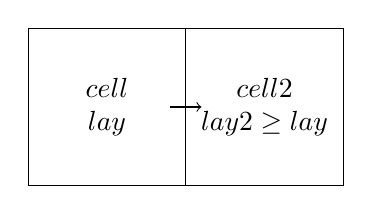
\begin{tikzpicture}[scale=2]
\draw(0,0)--(1,0)--(1,1)--(0,1)--cycle;
\node[align=center] at (0.5,0.5){$cell$\\$lay$};
\draw(1,0)--(2,0)--(2,1)--(1,1)--cycle;
\node[align=center] at (1.5,0.5){$cell2$\\$lay2\geq lay$};
\draw[->](0.9,0.5)--(1.1,0.5);
\end{tikzpicture}
}
\subcaptionbox{This is the case where the read is done in the same direction in negatif sign of the write.\label{code:fig:extrap:2}}{
\tikzset{external/export next=false}
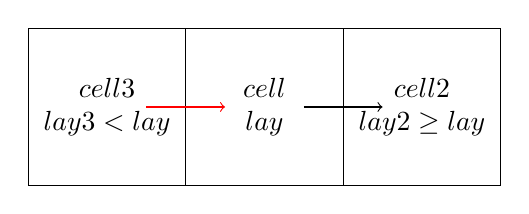
\begin{tikzpicture}[scale=2]
\draw(0,0)--(1,0)--(1,1)--(0,1)--cycle;
\draw(1,0)--(2,0)--(2,1)--(1,1)--cycle;
\draw(-1,0)--(0,0)--(0,1)--(-1,1)--cycle;
\draw[->](0.75,0.5)--(1.25,0.5);
\draw[->,red](-0.25,0.5)--(0.25,0.5);
\node[align=center] at (-0.5,0.5){$cell3$\\ $lay3<lay$};
\node[align=center] at (0.5,0.5){$cell$ \\$lay$};
\node[align=center] at (1.5,0.5){$cell2$ \\ $lay2\geq lay$};
\end{tikzpicture}
}
\subcaptionbox{This is the case where the read is done in the same direction in positif sign of the write.\label{code:fig:extrap:3}}
{
\tikzset{external/export next=false}
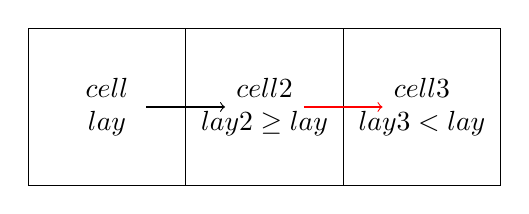
\begin{tikzpicture}[scale=2]
\draw(0,0)--(1,0)--(1,1)--(0,1)--cycle;
\draw(1,0)--(2,0)--(2,1)--(1,1)--cycle;
\draw(2,0)--(3,0)--(3,1)--(2,1)--cycle;
\draw[->](0.75,0.5)--(1.25,0.5);
\draw[->,red](1.75,0.5)--(2.25,0.5);
\node[align=center] at (2.5,0.5){$cell3$\\$lay3<lay$};
\node[align=center] at (1.5,0.5){$cell2$\\$lay2\geq lay$};
\node[align=center] at (0.5,0.5){$cell$\\$lay$};
\end{tikzpicture}
}
\subcaptionbox{This is the case where the read is done in a different direction of the write.\label{code:fig:extrap:4}}
{
\tikzset{external/export next=false}
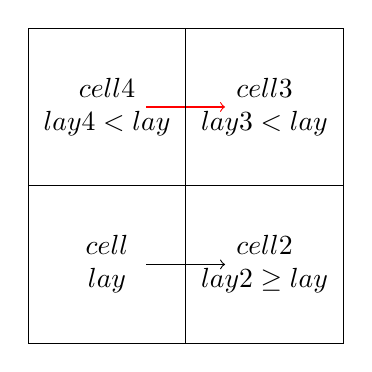
\begin{tikzpicture}[scale=2]
\draw(0,0)--(1,0)--(1,1)--(0,1)--cycle;
\draw(1,0)--(2,0)--(2,1)--(1,1)--cycle;
\draw[->](0.75,0.5)--(1.25,0.5);
\draw(0,1)--(1,1)--(1,2)--(0,2)--cycle;
\draw[->,red](0.75,1.5)--(1.25,1.5);
\draw(1,1)--(2,1)--(2,2)--(1,2)--cycle;
\node[align=center] at (0.5,1.5){$cell4$\\$lay4<lay$};
\node[align=center] at (1.5,1.5){$cell3$\\$lay3<lay$};
\node[align=center] at (0.5,0.5){$cell$\\$lay$};
\node[align=center] at (1.5,0.5){$cell2$\\$lay2\geq lay$};
\end{tikzpicture}
}
\caption{This are the case used in algorithm \ref{code:AlgorithmsExtrapolateNan1}. This are case where the speed component
is right the considered cell. In black is the speed component to set, in red is the speed component to read from.}
\end{center}
\end{figure}

\begin{figure}

\begin{center}
\subcaptionbox{The black speed component show a case considered when $lay$ has a given value.\label{code:fig:extrap:5}}
{
\tikzset{external/export next=false}
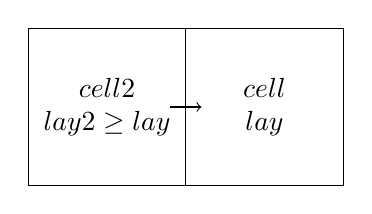
\begin{tikzpicture}[scale=2]
\draw(0,0)--(1,0)--(1,1)--(0,1)--cycle;
\node[align=center] at (0.5,0.5){$cell2$\\$lay2\geq lay$};
\draw(1,0)--(2,0)--(2,1)--(1,1)--cycle;
\node[align=center] at (1.5,0.5){$cell$\\$lay$};
\draw[->](0.9,0.5)--(1.1,0.5);
\end{tikzpicture}
}
\subcaptionbox{This is the case where the read is done in the same direction in positif sign of the write.\label{code:fig:extrap:6}}
{
\tikzset{external/export next=false}
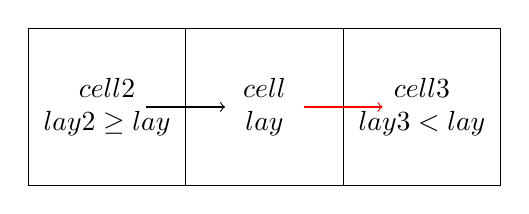
\begin{tikzpicture}[scale=2]
\draw(0,0)--(1,0)--(1,1)--(0,1)--cycle;
\draw(1,0)--(2,0)--(2,1)--(1,1)--cycle;
\draw(2,0)--(3,0)--(3,1)--(2,1)--cycle;
\draw[->](0.75,0.5)--(1.25,0.5);
\draw[->,red](1.75,0.5)--(2.25,0.5);
\node[align=center] at (2.5,0.5){$cell3$ \\ $lay3<lay$};
\node[align=center] at (1.5,0.5){$cell$\\$lay$};
\node[align=center] at (0.5,0.5){$cell2$ \\$lay2\geq lay$};
\end{tikzpicture}
}
\subcaptionbox{This is the case where the read is done in the same direction in negatif sign of the write.\label{code:fig:extrap:7}}
{
\tikzset{external/export next=false}
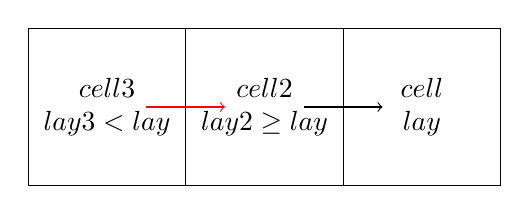
\begin{tikzpicture}[scale=2]
\draw(0,0)--(1,0)--(1,1)--(0,1)--cycle;
\draw(1,0)--(2,0)--(2,1)--(1,1)--cycle;
\draw(-1,0)--(0,0)--(0,1)--(-1,1)--cycle;
\draw[->](0.75,0.5)--(1.25,0.5);
\draw[->,red](-0.25,0.5)--(0.25,0.5);
\node[align=center] at (-0.5,0.5){$cell3$\\$lay3<lay$};
\node[align=center] at (0.5,0.5){$cell2$\\ $lay2\geq lay$};
\node[align=center] at (1.5,0.5){$cell$\\$lay$};
\end{tikzpicture}
}
\subcaptionbox{This is the case where the read is done in a different direction of the write.\label{code:fig:extrap:8}}
{
\tikzset{external/export next=false}
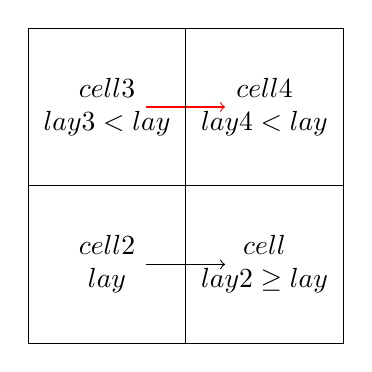
\begin{tikzpicture}[scale=2]
\draw(0,0)--(1,0)--(1,1)--(0,1)--cycle;
\draw(1,0)--(2,0)--(2,1)--(1,1)--cycle;
\draw[->](0.75,0.5)--(1.25,0.5);
\draw(0,1)--(1,1)--(1,2)--(0,2)--cycle;
\draw[->,red](0.75,1.5)--(1.25,1.5);
\draw(1,1)--(2,1)--(2,2)--(1,2)--cycle;
\node[align=center] at (0.5,1.5){$cell3$ \\ $lay3<lay$};
\node[align=center] at (1.5,1.5){$cell4$ \\ $lay4<lay$};
\node[align=center] at (0.5,0.5){$cell2$ \\ $lay$};
\node[align=center] at (1.5,0.5){$cell$\\ $lay2\geq lay$};
\end{tikzpicture}
}
\end{center}
\caption{This are the case used in algorithm \ref{code:AlgorithmsExtrapolateNan2}. This are case where the speed component
is left the considered cell. In black is the speed component to set, in red is the speed component to read from.}
\end{figure}

\begin{figure}

\begin{center}
\subcaptionbox{The black speed component show a case considered when $lay$ has a given value.\label{code:fig:extrap:9}}
{
\tikzset{external/export next=false}
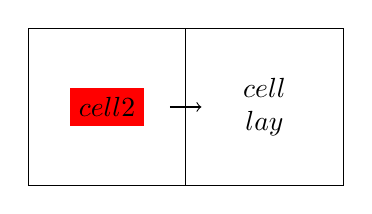
\begin{tikzpicture}[scale=2]
\draw(0,0)--(1,0)--(1,1)--(0,1)--cycle;
\node[align=center,fill=red] at (0.5,0.5){$cell2$};
\draw(1,0)--(2,0)--(2,1)--(1,1)--cycle;
\node[align=center] at (1.5,0.5){$cell$\\$lay$};
\draw[->](0.9,0.5)--(1.1,0.5);
\end{tikzpicture}
}
\subcaptionbox{This is the case where the read is done in the same direction in positif sign of the write.\label{code:fig:extrap:10}}
{
\tikzset{external/export next=false}
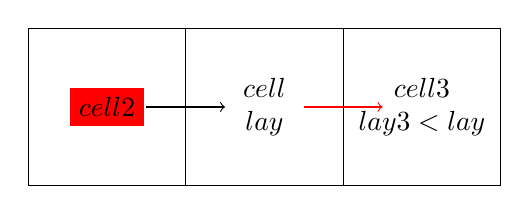
\begin{tikzpicture}[scale=2]
\draw(0,0)--(1,0)--(1,1)--(0,1)--cycle;
\draw(1,0)--(2,0)--(2,1)--(1,1)--cycle;
\draw(2,0)--(3,0)--(3,1)--(2,1)--cycle;
\draw[->](0.75,0.5)--(1.25,0.5);
\draw[->,red](1.75,0.5)--(2.25,0.5);
\node[align=center] at (2.5,0.5){$cell3$ \\ $lay3<lay$};
\node[align=center] at (1.5,0.5){$cell$\\$lay$};
\node[align=center,fill=red] at (0.5,0.5){$cell2$};
\end{tikzpicture}
}
\subcaptionbox{This is the case where the read is done in the same direction in negatif sign of the write.\label{code:fig:extrap:11}}
{
\tikzset{external/export next=false}
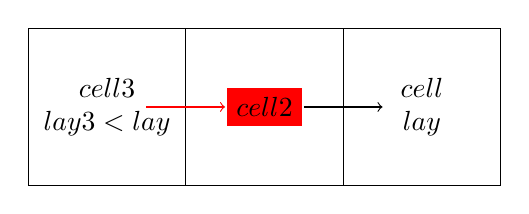
\begin{tikzpicture}[scale=2]
\draw(0,0)--(1,0)--(1,1)--(0,1)--cycle;
\draw(1,0)--(2,0)--(2,1)--(1,1)--cycle;
\draw(-1,0)--(0,0)--(0,1)--(-1,1)--cycle;
\draw[->](0.75,0.5)--(1.25,0.5);
\draw[->,red](-0.25,0.5)--(0.25,0.5);
\node[align=center] at (-0.5,0.5){$cell3$\\$lay3<lay$};
\node[align=center,fill=red] at (0.5,0.5){$cell2$};
\node[align=center] at (1.5,0.5){$cell$\\$lay$};
\end{tikzpicture}
}       
\subcaptionbox{This is the case where the read is done in a different direction of the write.\label{code:fig:extrap:12}}
{
\tikzset{external/export next=false}
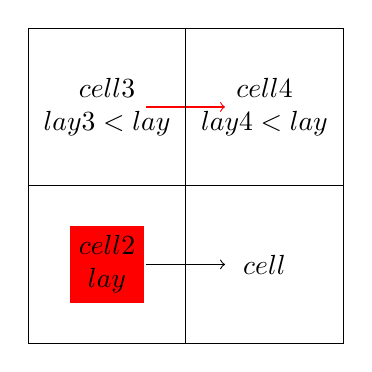
\begin{tikzpicture}[scale=2]
\draw(0,0)--(1,0)--(1,1)--(0,1)--cycle;
\draw(1,0)--(2,0)--(2,1)--(1,1)--cycle;
\draw[->](0.75,0.5)--(1.25,0.5);
\draw(0,1)--(1,1)--(1,2)--(0,2)--cycle;
\draw[->,red](0.75,1.5)--(1.25,1.5);
\draw(1,1)--(2,1)--(2,2)--(1,2)--cycle;
\node[align=center] at (0.5,1.5){$cell3$ \\ $lay3<lay$};
\node[align=center] at (1.5,1.5){$cell4$ \\ $lay4<lay$};
\node[align=center,fill=red] at (0.5,0.5){$cell2$ \\ $lay$};
\node[align=center] at (1.5,0.5){$cell$};
\end{tikzpicture}
}
\end{center}
\caption{This are the case used in algorithm \ref{code:AlgorithmsExtrapolateNan3}. This are case where the speed component
is left the considered cell but where the left cell doesn't exist. In black is the speed component to set, in red is the speed component to read from. The cell marked in red doesn't exist, we cannot access left and below speed of them.}
\end{figure}
\subsection{Interpolation}

We will now show the pseudo code for interpolation for $N$ dimension white $N$-linear interpolation.
The principal difficulty is that on a staggered grid the position of know speed vary for all component.
The algorithm needed to do the translation is shown in algorithm \ref{code:GetSpeed}.
The interpolation is show in algorithm \ref{code:GetSpeedImpl}.

\begin{algorithm}
\caption{Algorithm witch calculate recursively the interpolation for scaled position in the square in range $[0,1]\times[0,1]$.}
\label{code:GetSpeedImpl}
\begin{algorithmic}[1]
\Function{GetSpeedImpl}{$posscal,i,cell,k$}\Comment{Get the interpolated speed in direction $k$ at position $posscal$ for cell $cell$.
$i$ is the recursif parameter it's first value should be 1.}
\State $cell2 \gets cell.\FuncCall{GetNeighbour}(i,1)$\Comment{We set $cell2$ to access speed in the other side in direction $i$.}
		\If{$i<dim$}\Comment{We are not in a terminal case, we do a linear interpolation in direction $i$ and recurse the linear interpolation in the rest
		of the dimension. The cell variable $cell2$ is used because it's ``origine'' of the second function call.}
			\State $ret \gets (1-posscal.\FuncCall{Get}(i))\cdot \FuncCall{GetSpeedImpl}(posscal,i+1,cell,k)+posscal.\FuncCall{Get}(i)\cdot \FuncCall{GetSpeedImpl}(posscal,i+1,cell2,k)$
			\State \Return $ret$
		\Else \Comment{We are in a terminal case. We acess the speed and do the linear interpolation.}
			\State $ret\gets (1-posscal.\FuncCall{Get}(i))*(cell.\FuncCall{SpeedGet}(k))+posscal.\FuncCall{Get}(i)*(cell2.\FuncCall{SpeedGet}(k))$
			\State \Return $ret$
		\EndIf
\EndFunction
\end{algorithmic}
\end{algorithm}

\begin{algorithm}
\caption{Algorithm witch interpolate the speed at a given position.}
\label{code:GetSpeed}
\begin{algorithmic}[1]
\Function{GetSpeed}{$pos$}
		\For{$i=1 \To dim$}
			\State $posdelta.\FuncCall{Set}(i,\frac{pos.\FuncCall{Get}(i)}{h.\FuncCall{Get}(i)})$
			\Comment{Scale the position.}
			\State $key0.\FuncCall{Set}(i,round(pos_delta.GetRef(i)))$
			\Comment{We round to the nearest integer to find in witch integer cell is the particle.}
			\State $posdelta.\FuncCall{Set}(i,posdelta.\FuncCall{Get}(i)-key0.\FuncCall{Get}(i))$
			\Comment{Because we have rounded to the nearest integer the value of $posdelta$ are in $[-0.5,0.5[$ 
			(the exact up or down rounding depend on the specification of the rounding function).}
		\EndFor
		\For{$k=1\To dim$}\Comment{For every speed component.}
			\State $posdelta.\FuncCall{Set}(k,posdelta.\FuncCall{Get}(k)+0.5)$\Comment{Because we are in a staggered grid the position is translated.
			The $0$ vector is at cell center. The range of $posdelta.\FuncCall{Get}(k)$ is in range $[0,1[$.}
			\For{$j=1 \To dim$}
				\If{$j\neq k$}\Comment{We loop on every speed component different than the used one.}
					\If{$posdelta.\FuncCall{Get}(j)<0$}\Comment{$posdelta.\FuncCall{Get}(j)$ is in range $[-0.5,0.5[$.}
						\State $key.\FuncCall{Set}(j,key0.\FuncCall{GetRef}(j)-1)$ \Comment{We go to the cell below because we have rounded to the cell above.}
						\State $posdelta2.\FuncCall{Set}(j,1+posdelta.\FuncCall{Get}(j))$ \Comment{We change the $posdelta2$ to the translation.
						$posdelta2.\FuncCall{Get}(j)$ is now in range $[0,1[$.}
					\Else
						\State $key.\FuncCall{Set}(j,key0.\FuncCall{Get}(j))$
						\State $posdelta2.\FuncCall{Set}(j,posdelta.\FuncCall{Get}(j))$
					\EndIf
				\Else
					\State $key.\FuncCall{Set}(j,key0.\FuncCall{Get}(j))$
					\State $posdelta2.\FuncCall{Set}(j,posdelta.\FuncCall{Get}(j))$
				\EndIf
			\EndFor
			\State $cell\gets Grid[key]$\Comment{We get the cell at the calculated $key$.}
			\State $ret.\FuncCall{Set}(k,\FuncCall{GetSpeedImpl}(pos_delta2,1,cell,k))$ \Comment{We call the interpolation routine and set the result in the return vector.}
			\State $posdelta.\FuncCall{Set}(k,posdelta.\FuncCall{Get}(k)-0.5)$
		\EndFor
		\State \Return $ret$
	\EndFunction
\end{algorithmic}
\end{algorithm}


\subsection{Conclusion}

We have seen there all algorithm for extrapolation and cell initialization.
The rest are the numerical step show in section \ref{splitting} or \ref{differentialequation} 
and in the previous chapter.

\section{Numerical experiment}

\subsection{One particle fall}

We have discussed this case qualitatively we will now simulated it numerically.

We take as initial condition a single particle with 0 speed everywhere without viscosity falling from gravity.

The analytical solution is for the continuous problem given by:
\begin{align}
v&=-gt\\
x&=x_0-\frac{1}{2}gt^2
\end{align}

If we add viscosity the same is true.

\subsubsection{Result}

We see in figure \ref{topo:singl_part:fig1} that the none splitted method coincide with the analytical solution for as
integration method Runge-Kutta of order 4. The reason is that the analytical solution is a polynomial of order 2.

At the contrary because of the splitting a splitting method will incorrectly approximate the result, because it's of order 1 at general.

When we have big time step like $\alpha=2$ none splitted method behave better. But it's important to recall the result on fixed grid,
that having a too big time step make diverge.

\begin{figure}
\begin{tikzpicture}
	\begin{axis}[width=\textwidth,use units,x unit=\second,y unit=\meter,xlabel=$t$ Position,ylabel=$y$ Position,no markers]
		\addplot table[col sep=comma,x=t,y=y]{topology/single_part/traj1.csv};
		\addlegendentry{Splitted $\alpha=0.1$}
		\label{top:single_part:traj1}
		\addplot table[col sep=comma,x=t,y=y]{topology/single_part/traj2.csv};
		\label{top:single_part:traj2}
		\addlegendentry{None Splitted $\alpha=0.1$}
		\addplot[green] table[col sep=comma,x=t,y=y]{topology/single_part/traj3.csv};
		\addlegendentry{Splitted $\alpha=2$}
		\label{top:single_part:traj3}
		\addplot[purple] table[col sep=comma,x=t,y=y]{topology/single_part/traj4.csv};
		\label{top:single_part:traj4}
		\addlegendentry{None Splitted $\alpha=2$}
		\addplot[domain=0:2,dotted] gnuplot{-x*x*9.81/2};
		\label{top:single_part:anal1}
		\addlegendentry{Analytical}
	\end{axis}
\end{tikzpicture}
\caption{Comparison between splitting and not splitting for a single particle problem. 
The integration method is Runge-Kutta of order 4 for the two case.
We see that the none splitting method (\ref{top:single_part:traj2} and \ref{top:single_part:traj4}) is a very good approximation to the analytical solution (\ref{top:single_part:anal1}).
Instead the splitting method (\ref{top:single_part:traj1} and \ref{top:single_part:traj3}) is different than the analytical solution (\ref{top:single_part:anal1}).
For the two methods, we have used $\Delta x=0.01$. The time step limiter was a maximal time step $dt_{max}=0.01$.
}
\label{topo:singl_part:fig1}
\end{figure}

\subsection{Lateral Jet}

We consider a continuous source of speed in the $x$ direction. With gravity at the $y$ direction.
The analytical solution can be found without consideration of the boundary condition.

A single particle with initial $x$ speed $v_{0}$ witch go from position $y$ $y_0$ and with initial time $t_0$.

The speed is:
\begin{align}
	v_{x}&=v_{0}\\
	v_{y}&=-\frac{g}{2}(t-t_0)^2
\end{align}

The position of the particle is then:
\begin{align}
	x&=v_{0}(t-t_0)\\
	y&=y_0-\frac{g}{2}(t-t_0)^2
\end{align}

We will now try to define the speed in a particle manner.
The time is given by:
\begin{equation}
	t-t_{0}=\frac{x}{v_{0}}
\end{equation}

The speed is then given by:
\begin{align}
	v_{x}&=v_{0}\\
	v_{y}&=-\frac{g}{2}\frac{x^2}{v_{0}}
\end{align}

This is divergence free.
So we are a solution of the Navier-Stokes equation.

But we doesn't respect the boundary condition.

We cannot know apriori if the numerical solution with correct boundary solution will respect this solution.
But we can expect that a perturbation at boundary that will respect the boundary condition,
will rest in the boundary and not enter in the fluid.

This approximation is called Boundary Layer.


We see in figure \ref{topo:extrap:lateral:8_1}, \ref{topo:extrap:lateral:9_1} and \ref{topo:extrap:lateral:10_1} that lateral
speed are smirred by the viscosity and is quasi constant witch is the analytical solution.

The boundary of the analytical solution is near to the numerical solution.
Only the end of the fluid don't follow the analytical solution.
This indicate that boundary layer is a correct approximation.

\subsubsection{Result}
\begin{figure}
	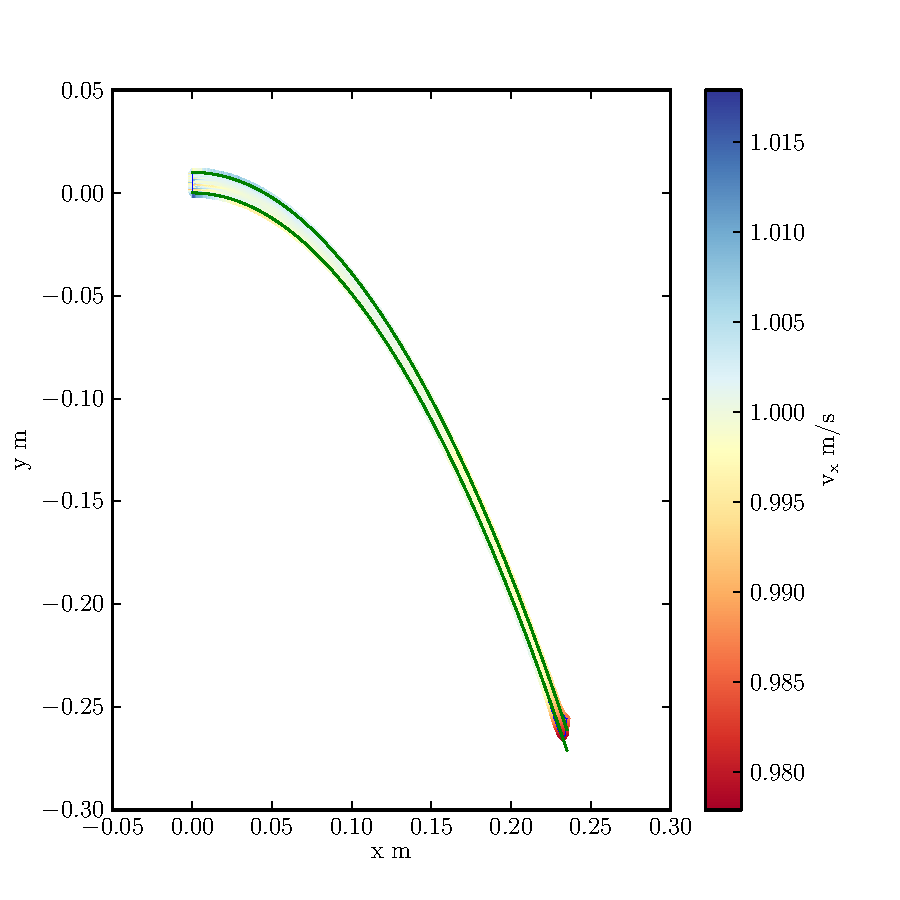
\includegraphics{topology/lateral_jet/plot_8__1_186.pdf}
	\caption{None splitted result with Runge-Kutta rk4 with $\nu=1.307e-6$ $\alpha=0.5$.
	This is the $x$ speed.
	The green line is the analytical solution boundary for the result without boundary condition.
	The blue line is the calculate boundary.
	We see that except at the end, the two coincide.
	At interior the speed take the analytical value witch is constant and has a little jump in the boundary.
	The perturbation at initial condition are smirred by the viscosity.}
	\label{topo:extrap:lateral:8_1}
\end{figure}

\begin{figure}
	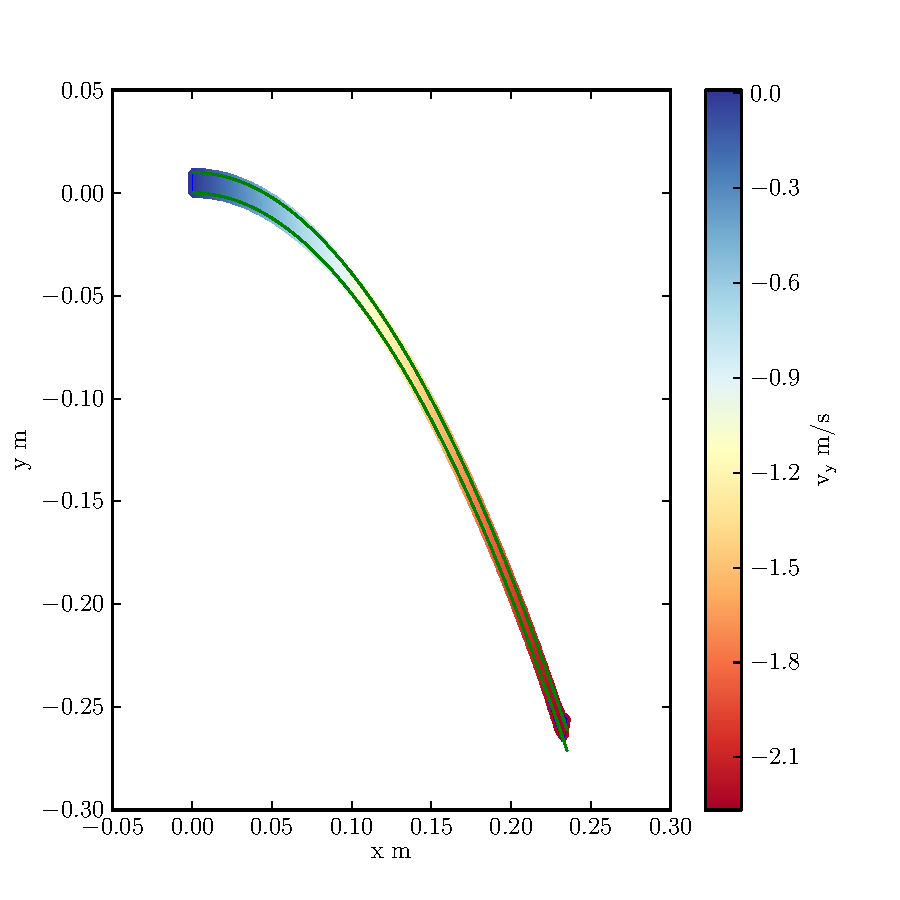
\includegraphics{topology/lateral_jet/plot_8__2_186.pdf}
	\caption{None splitted result with Runge-Kutta rk4 with $\nu=1.307e-6$ $\alpha=0.5$.
	This is the $y$ speed.
	The green line is the analytical solution boundary for the result without boundary condition.
	The blue line is the calculate boundary.
	We see that except at the end, the two coincide.
	The $y$ speed is proportional to the $x^2$ position, witch coincide with the analytical result.
	The perturbation at initial condition are smirred by the viscosity.}
	\label{topo:extrap:lateral:8_2}
\end{figure}

\begin{figure}
	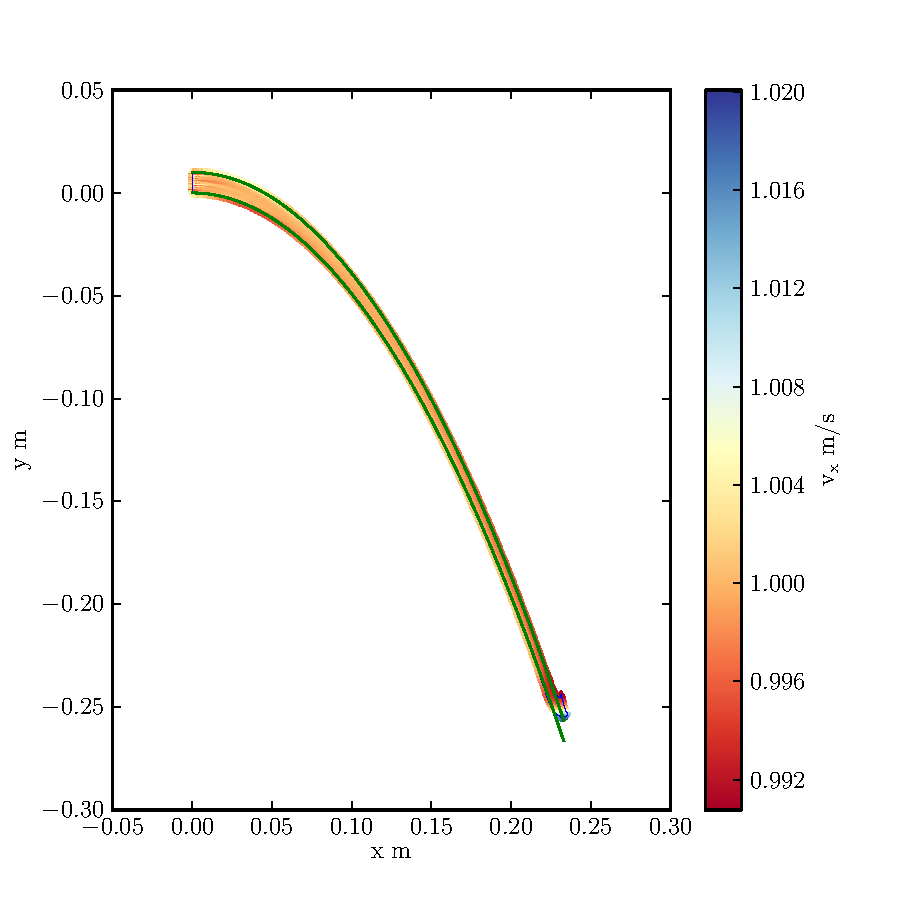
\includegraphics{topology/lateral_jet/plot_9__1_182.pdf}
		\caption{Splitted result with Runge-Kutta rk4 with $\nu=1.307e-6$ $\alpha=0.5$.
	This is the $x$ speed.
	The green line is the analytical solution boundary for the result without boundary condition.
	The blue line is the calculate boundary.
	We see that except at the end, the two coincide.
	At interior the speed take the analytical value witch is constant and has a little jump in the boundary.
	The perturbation at initial condition are smirred by the viscosity.}
	\label{topo:extrap:lateral:9_1}
\end{figure}

\begin{figure}
	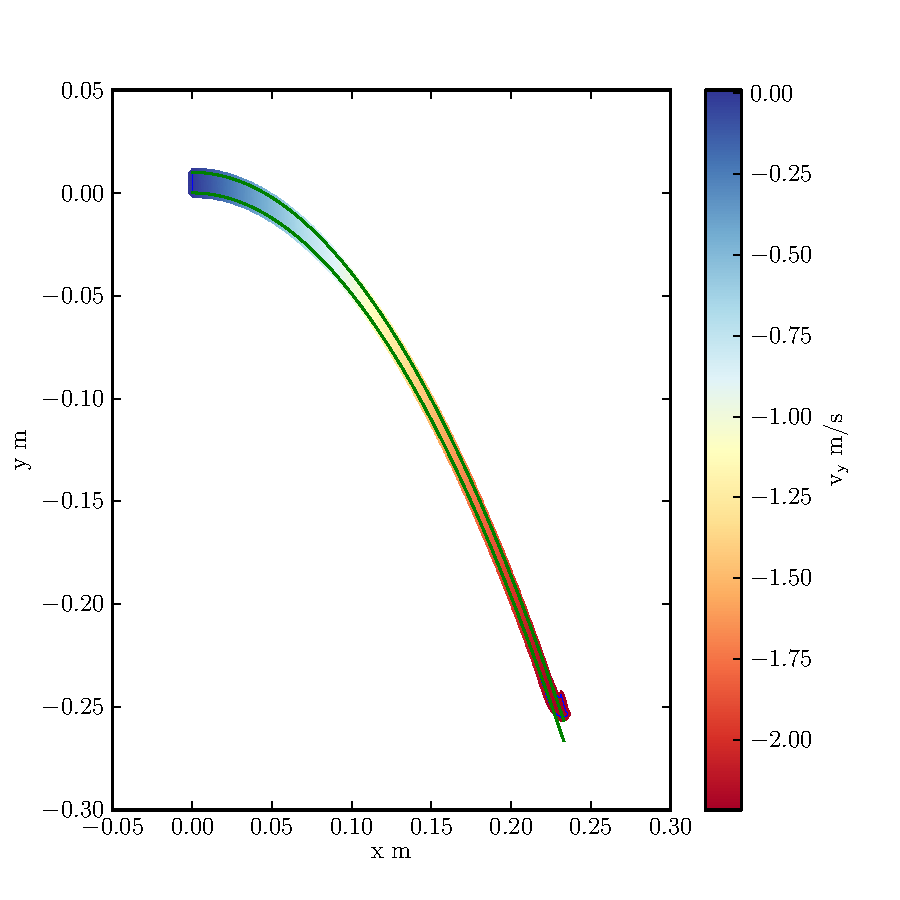
\includegraphics{topology/lateral_jet/plot_9__2_182.pdf}
		\caption{Splitted result with Runge-Kutta rk4 with $\nu=1.307e-6$ $\alpha=0.5$.
	This is the $y$ speed.
	The green line is the analytical solution boundary for the result without boundary condition.
	The blue line is the calculate boundary.
	We see that except at the end, the two coincide.
	The $y$ speed is proportional to the $x^2$ position, witch coincide with the analytical result.
	The perturbation at initial condition are smirred by the viscosity.}
	\label{topo:extrap:lateral:9_2}
\end{figure}


\begin{figure}
	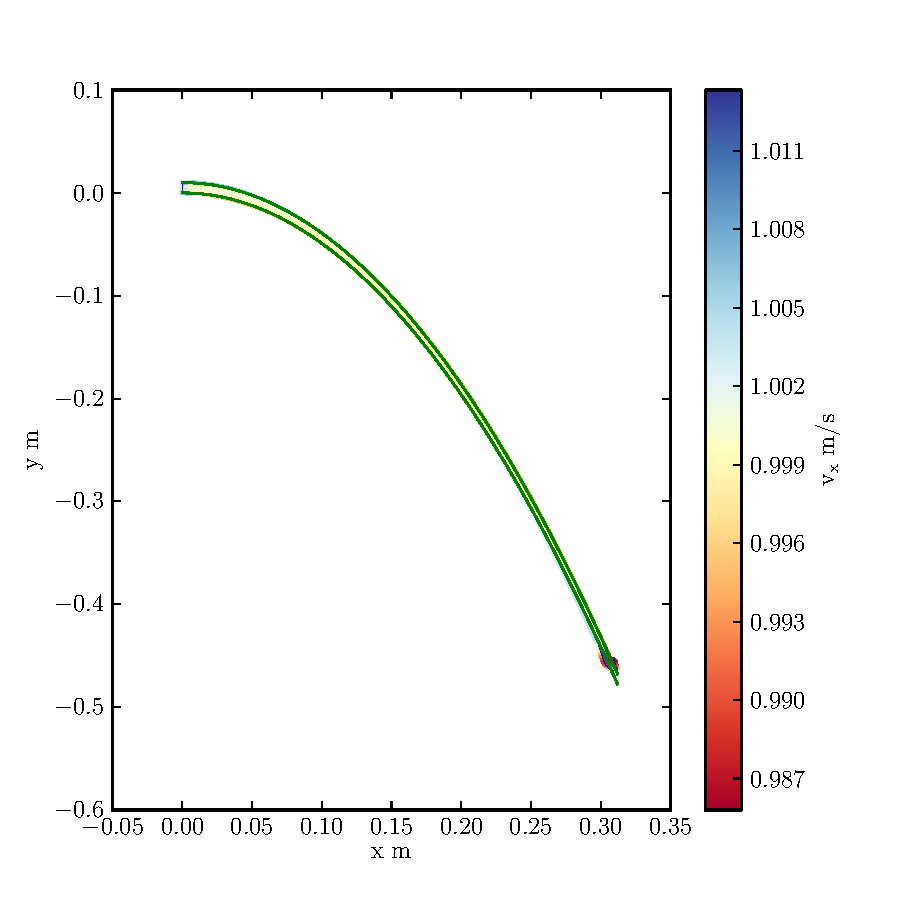
\includegraphics{topology/lateral_jet/plot_10__1_293.pdf}
			\caption{Splitted result with Euler with $\nu=1.307e-6$ $\alpha=0.5$.
	This is the $x$ speed.
	The green line is the analytical solution boundary for the result without boundary condition.
	The blue line is the calculate boundary.
	We see that except at the end, the two coincide.
	At interior the speed take the analytical value witch is constant and has a little jump in the boundary.
	The perturbation at initial condition are smirred by the viscosity.}
	\label{topo:extrap:lateral:10_1}
\end{figure}

\begin{figure}
	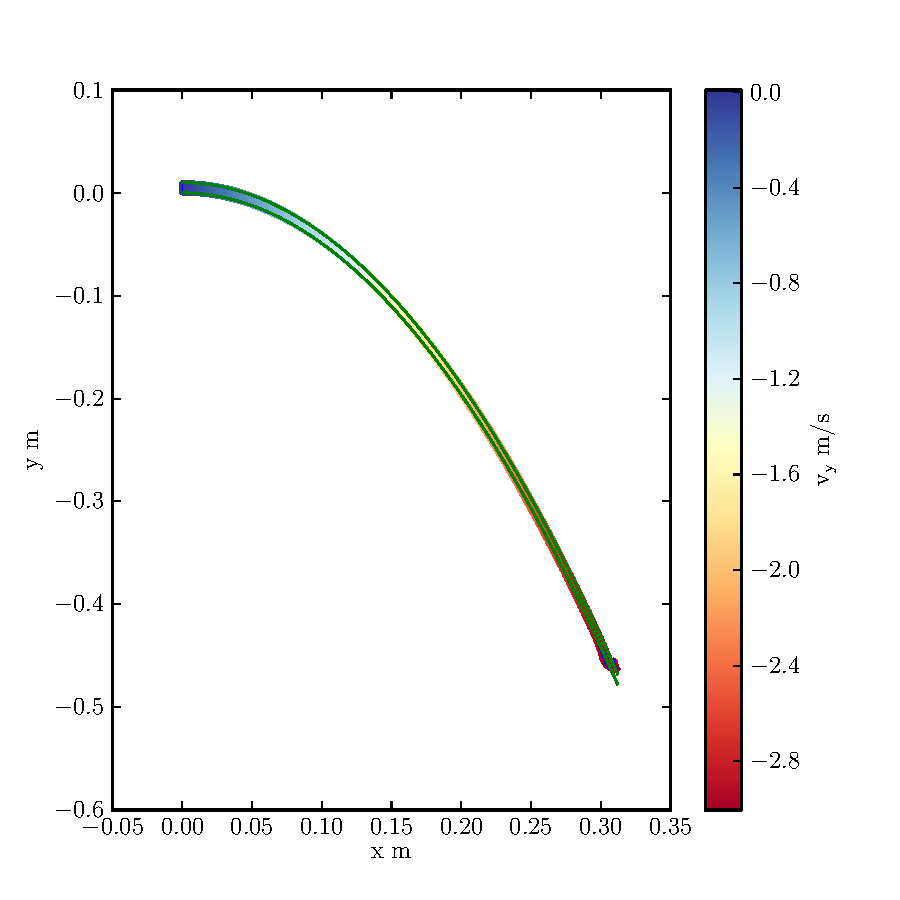
\includegraphics{topology/lateral_jet/plot_10__2_293.pdf}
			\caption{Splitted result with Euler with $\nu=1.307e-6$ $\alpha=0.5$.
	This is the $y$ speed.
	The green line is the analytical solution boundary for the result without boundary condition.
	The blue line is the calculate boundary.
	We see that except at the end, the two coincide.
	The $y$ speed is proportional to the $x^2$ position, witch coincide with the analytical result.
	The perturbation at initial condition are smirred by the viscosity.}
	\label{topo:extrap:lateral:10_2}
\end{figure}


